\documentclass{FastFyp}
\begin{document}
\raggedbottom
\newcommand{\supervisor}{Dr. Ammar Haider \\ Co-Supervisor: Ms. Nosheen Manzoor}
\newcommand{\university}{National University of Computer and Emerging Sciences, Lahore}
\newcommand{\fyptitle}{PhishHook: Lightweight Client-Side Phishing Detection using Hybrid Approach}
\newcommand{\degree}{BS}
\newcommand{\Studentone}{Abdullah Shahbaz     23L-0874    BS(CS)}
\newcommand{\Studenttwo}{Muhammad Hassan Raza     23L-3049    BS(CS)}
\newcommand{\Studentthree}{Muhammad Ibrahim     23L-0837    BS(CS)}
\date{\today}
\renewcommand{\contentsname}{Table of Contents}

\makeatletter
    \begin{titlepage}
        
\includegraphics[width=0.2\linewidth]{Figures/nulogo.png}\hfill
        
\includegraphics[width=0.2\linewidth]{Figures/fast.png}\\
        \begin{center}
            {\large\bfseries \university}\\[7ex]
            
\includegraphics[width=0.4\linewidth]{Figures/fastlogo.png}\\[8ex]
            {\huge \bfseries  \fyptitle }\\[10ex]
            {\Studentone}\\{\Studenttwo}\\{\Studentthree}\\[4ex]
            {Supervisor: \supervisor} \\ [10ex]
            {Final Year Project}\\
            {\large \@date}
        \end{center}
    \end{titlepage}
\makeatother
\frontmatter

\newpage \thispagestyle{empty} \mbox{} \newpage

\pagestyle{empty}


\newcommand{\signatureline}[1]{%
    \parbox[t]{6cm}{\raggedleft
        \includegraphics[height=1.8cm]{#1}\\[-0.3cm]
        \makebox[6cm]{\dotfill}%
    }%
}

\section*{\begin{center}{Anti-Plagiarism Declaration} \end{center}}
This is to declare that the above publication was produced under the:
\begin{flushleft}
\bf Title: \fyptitle
\end{flushleft}

is the sole contribution of the author(s), and no part hereof has been reproduced as it is the basis (cut and paste) that can be considered Plagiarism. All referenced parts have been used to argue the idea and cited properly. I/We will be responsible and liable for any consequence if a violation of this declaration is determined.
\\[4ex]
Date: \today

\begin{flushright}
Name: Abdullah Shahbaz
\\[1ex]
\signatureline{Figures/signature_abdullah.png}
\\[5ex]
Name: Muhammad Hassan Raza
\\[1ex]
\signatureline{Figures/signature_hassan.png}
\\[5ex]
Name: Muhammad Ibrahim
\\[1ex]
\signatureline{Figures/signature_ibrahim.png}
\end{flushright}
\vspace{1 cm}
\hrule
\vspace{0.5 cm}

\section*{Author's Declaration}
This states Authors' declaration that the work presented in the report is their own, and has not been submitted/presented previously to any other institution or organization.
\pagebreak

\section*{Abstract}
Phishing remains a persistent threat, yet the majority of detection systems are based on an inference from cloud usage or external reputation checks, or very heavy models that raises privacy and performance issues. This research and development project presents PhishHook, a lightweight, privacy-preserving phishing detection extension for Chromium browsers (Manifest V3) that performs all analysis on the user's device, using only the URL string and the already-rendered page content, with no network lookups and no off-device data transmission.

For web pages, PhishHook combines two complementary modules. An unsupervised URL anomaly model, trained on benign URLs only, assigns each URL an anomaly score without requiring labelled phishing examples during training. A quantised MobileBERT classifier, trained on text derived from the page's DOM (title, form fields, link domains and visible text), produces a phishing probability. A small logistic-regression model fuses the percentile-ranked URL score and the calibrated DOM score into a single risk score, trained on a partition held out from DOM training to prevent leakage. For email, a MobileBERT teacher is used only during training to distil knowledge into a compact BiLSTM student, which is the only email model deployed and which reads only content visible in the webmail interface.

The study investigates how well the unsupervised URL module detects phishing compared with a supervised reference baseline, how accurate and robust the quantised DOM classifier is, whether fusion reduces false alarms compared with either module alone, which input components contribute most, and whether distillation improves the email student over the same model trained without it. 

\vspace{0.5em}



\pagebreak

\section*{Executive Summary}
Phishing remains one of the most persistent and financially damaging forms of cyber attack. Attackers create new phishing pages within hours, and traditional defences struggle to keep up. Blocklists only detect threats that have already been reported, cloud-based detection systems require sending user traffic to a remote server, and many deep learning models are too heavy to run inside a browser. PhishHook addresses these limitations by performing phishing detection entirely on the user's device, inside a Chromium Manifest V3 extension, using only the URL string and the already-rendered DOM of the page the user has loaded.

The purpose of this document, as discussed in the first chapter, is to present the design, implementation, and evaluation of PhishHook. The project aims to build a lightweight, privacy-preserving extension that detects both web and email phishing without any network lookups and without transmitting user data off the device. The document describes the problem domain, the research questions, and the specific contributions of the project relative to PhishLang, which serves as its base paper.

The second chapter presents the project vision. It defines the problem, the goals and objectives of the project, the scope, the alignment with Sustainable Development Goals, and the stakeholders. The chapter states clearly which parts of the project are the core study and which are narrower in scope. The web pipeline, comprising an unsupervised URL module, a supervised DOM classifier, a fusion model, and dynamic monitoring, is the full study. The email pipeline, using knowledge distillation from a MobileBERT teacher into a compact BiLSTM student, is a narrower study.

The third chapter provides a detailed literature review. It surveys prior work across five categories: unsupervised URL anomaly detection, supervised transformer-based web phishing detection, hybrid and fusion-based approaches, email phishing detection with knowledge distillation, and client-side lightweight deployment. Each reviewed paper is summarised, critically analysed, and related to PhishHook. The chapter closes with a summary table that captures the methods, results, and limitations of the reviewed works.

The fourth chapter presents the Software Requirement Specifications. It lists the major features of the system, the functional and non-functional requirements, the quality attributes, the assumptions, the use cases, the hardware and software requirements, the graphical user interface, and the risk analysis. Each requirement is linked to a specific user-facing or system-facing behaviour, so that the design and the implementation can be verified against it.

The fifth chapter describes the proposed approach and methodology. It presents the datasets and how they are divided into training, tuning, calibration, and test partitions, with explicit rules to prevent leakage. It then describes the entirely-local input design, the URL and DOM parsing procedures, the unsupervised URL anomaly module with its three candidates (Isolation Forest, character-level autoencoder, and a K-Means baseline), the supervised DOM classifier with MobileBERT and its comparison against LightGBM, the fusion meta-classifier, and the email knowledge distillation pipeline. The chapter also defines the evaluation protocol, the statistical tests, the resource measurement protocol, and the adversarial evaluation.

The sixth chapter provides the high-level and low-level design of PhishHook. It describes the system architecture, the subsystem architecture of each of the five modules, the architectural strategies adopted, the class diagram, the sequence diagrams, and the policies and tactics that govern the implementation. The diagrams show how data flows between the content script, the service worker, the offscreen document, and the WebAssembly runtime.

To conclude, PhishHook aims to advance the state of lightweight, privacy-preserving phishing detection by combining an unsupervised URL module, a supervised DOM classifier, a fusion meta-classifier, dynamic post-load monitoring, and a distilled email detector, all running entirely on the user's device. The project is designed to be reproducible, honest about its limitations, and practical to deploy in a standard Chromium browser.
\pagebreak

\pagestyle{fancy}
\tableofcontents

\pagebreak
\listoffigures
\addcontentsline{toc}{chapter}{List of Figures}
\pagebreak
\listoftables
\addcontentsline{toc}{chapter}{List of Tables}

\mainmatter

% ============================================================
% CHAPTER 1: INTRODUCTION
% ============================================================
\chapter{Introduction}
\label{ch:intro}
Phishing is still one of the most prolific and adaptive threats in cybersecurity. Traditional defenses are being foiled by attackers because they use dynamic webpage behavior, post-load DOM manipulation and AI-generated email content. Only known threats will be caught by blocklists and cloud-based detection will have latency, user privacy and connection dependency problems. PhishHook addresses these limitations by performing phishing detection entirely on the user's device, inside a Chromium Manifest V3 extension, using only the URL string and the already-rendered DOM of the page the user has loaded. All of the working is done in Chrome and data never leave the user device. 

PhishHook uses a dual framework web pipeline. A lightweight unsupervised model analyses the URL string and assigns an anomaly score, on the premise that phishing URLs deviate from patterns learned from benign URLs only. In parallel, a supervised quantised MobileBERT model analyses DOM-derived text (title, form fields and labels, link domains, and visible text) and produces a calibrated phishing probability. A small L2-regularised logistic-regression meta-classifier fuses the two scores into a single risk assessment. For email, a MobileBERT teacher is fine-tuned offline and distilled into a compact BiLSTM student only the student is deployed, and it consumes only what is visible in the webmail DOM. This report provide details of the design, implementation and evaluation of this pipeline,
It includes the entirely-local input design, the unsupervised URL anomaly module, the supervised DOM module, the fusion method, the distillation methodology for email and its analysis for the MV3 deployment.


\section{Purpose of this Document}
The purpose of this document is to present the design, implementation, and evaluation of our FYP, PhishHook which addresses the growing problem of phishing attacks that bypass traditional blocklists and cloud-based detectors. Nowadays, phishing pages can be created, and edited in a matter of hours and cloud based detection methods create privacy and network dependency issues. Old and privacy-compromising detection strategies put customers at risk of credential theft and financial fraud. Legacy and privacy-compromising detection strategies put customers at risk of credential theft and financial fraud. Our project uses a dual framework approach for this challenge as a client-side solution that can be integrated directly into a Chromium Manifest V3 browser extension to detect anomalies in URLs using unsupervised learning, classify the DOM using supervised learning and knowledge distillation without any data being sent off-device.

The research questions we aim to explore are: (RQ1) How well does an unsupervised URL anomaly model, trained on benign URLs only, detect phishing URLs at realistic base rates, and how does it compare with a supervised URL baseline used only as a reference? (RQ2) Which parts of the URL and DOM input contribute most to detection, and what is the accuracy-versus-resource trade-off inside the browser? (RQ3) On the same information extracted from the rendered DOM, does a quantised MobileBERT classifier detect phishing more reliably than a LightGBM model trained on engineered features, particularly on unseen sources and later time periods at low false-alarm rates?

Through this endeavour, we aspire to advance the state of lightweight, privacy-preserving phishing detection and to provide a practical, reproducible framework that future researchers and browser extension developers can build upon. This report presents the methodology, design, implementation, testing, and evaluation of PhishHook, together with its limitations, threat model, and future work.  


\section{Contributions over PhishLang}
\label{sec:contributions}
PhishHook builds on PhishLang \cite{phishlang2026}, which established the feasibility of fully client-side phishing detection using MobileBERT over actionable HTML elements. The concrete contributions of PhishHook relative to PhishLang are described in the following subsections.

\subsection{URL-Excluded DOM Input}
PhishHook deliberately excludes the page URL from the supervised DOM model, so that the URL module and the DOM module are complementary and so that the input-contribution ablation (RQ2) is meaningful. PhishLang uses actionable HTML elements but does not enforce this separation.

\subsection{Unsupervised URL Anomaly Module}
PhishHook adds a second, unsupervised path that scores the URL string without any labelled phishing data during training, selecting the deployed model by a pre-registered rule. PhishLang is a single supervised model.

\subsection{Dynamic Monitoring}
PhishHook continuously monitors the rendered DOM for security-relevant changes after page load, such as new forms appearing, form destinations being modified, or significant script changes. This addresses a documented limitation of PhishLang, which performs static analysis of page source code at the moment of access but does not observe post-load DOM mutations or dynamically injected phishing elements.

\subsection{Distilled Email Detector}
PhishHook adds a separate email pipeline using knowledge distillation from an offline MobileBERT teacher into a deployed BiLSTM student. PhishLang does not address email. This is treated as a stretch goal in the project scope.

\section{Intended Audience}
This document is intended for the following readers:
\begin{itemize}
    \item \textbf{Project supervisor and panel of evaluators}, who will use it to assess the problem definition, the technical approach, and the completeness and quality of our work.

    \item \textbf{End users}, such as general internet users, students, and professionals, who want to understand what PhishHook does, what it protects them from, what its limitations are (for example, post-load detection and the residual limitations of an entirely-local unsupervised URL module), and how their privacy is preserved because no data leaves their device.
 

\end{itemize}

\section{Definitions, Acronyms, and Abbreviations}
\begin{itemize}
    \item \textbf{PhishHook:} The lightweight, client-side phishing detection framework proposed in this FYP.
    \item \textbf{Unsupervised URL Module:} The anomaly-detection component that scores URLs without any labelled phishing data during training.
    \item \textbf{Character-Level Autoencoder:} A neural network trained to reconstruct benign URL character sequences; high per-character reconstruction error indicates anomalous (potentially phishing) URLs.
    \item \textbf{Isolation Forest:} An ensemble anomaly-detection method that isolates observations using random splits; used on engineered lexical URL features.
    \item \textbf{Reconstruction Error:} The mean per-character error between the input URL and the autoencoder's reconstructed output over non-padded positions; used as the anomaly score.
    \item \textbf{Anomaly Score:} A scalar produced by the URL module; higher values indicate greater deviation from benign patterns.
    \item \textbf{Engineered Lexical Features:} Hand-crafted URL statistics computed separately over host, path, and query (for example URL length, digit ratio, Shannon entropy, subdomain depth, path depth, query-parameter count, hyphen count in host, dot count in host, longest digit run, presence of punycode, presence of percent-encoding, TLD frequency rank, and rare-TLD flag).
    \item \textbf{Supervised DOM Module:} The classification component trained on labelled (phishing or benign) DOM-derived text.
    \item \textbf{MobileBERT:} A lightweight transformer-based language model. Used as the supervised DOM classifier (deployed, quantised) and as the teacher for email distillation (offline only).
    \item \textbf{DOM-Derived Text:} Text extracted from the rendered DOM (title, form fields and labels, link domains, visible text) in a defined priority order within the 512-token limit. The URL is excluded from this input.
    \item \textbf{Fusion Meta-Classifier:} A small L2-regularised logistic-regression model that combines the percentile-ranked URL anomaly score and the temperature-calibrated DOM logit into a single risk score.
    \item \textbf{Held-Out Partition:} A data partition (P3) that is excluded from DOM training, so that DOM scores on it are out-of-sample by construction. Used to fit the fusion meta-classifier without leakage.
    \item \textbf{Temperature Calibration:} Post-hoc scaling of model logits so that predicted probabilities better reflect true likelihoods; fitted on the outputs of the quantised deployed DOM model, because quantisation changes the logits.
    \item \textbf{Percentile Rank Transformation:} Mapping a raw anomaly score to its percentile against a frozen set of benign validation scores produced by the quantised deployed URL model; ensures that the URL and DOM inputs to fusion are on comparable scales.
    \item \textbf{BiLSTM:} Bidirectional Long Short-Term Memory; the student model for email phishing detection, deployed in the extension.
    \item \textbf{Knowledge Distillation:} A training technique in which a large teacher model transfers knowledge to a smaller student model.
    \item \textbf{Teacher Model:} The fine-tuned MobileBERT used offline to produce soft labels for the email student; not deployed.
    \item \textbf{Student Model:} The distilled BiLSTM exported and deployed for email phishing detection.
    \item \textbf{Soft Labels:} The probability distribution produced by the teacher, used to train the student.
    \item \textbf{Temperature (T):} A scaling parameter applied to teacher logits to soften the soft-label distribution during distillation.
    \item \textbf{KL Divergence:} Kullback--Leibler divergence, used as the distillation loss between teacher and student distributions.
    \item \textbf{ONNX:} Open Neural Network Exchange, the model export format used for the URL autoencoder, the DOM MobileBERT, and the email BiLSTM. The Isolation Forest is exported as a JSON tree dump with a JS evaluator, and the fusion meta-classifier is implemented as plain JavaScript constants.
    \item \textbf{Offscreen Document:} A Chromium MV3 API that allows DOM-capable, long-running work outside the service worker.
    \item \textbf{Quantisation:} Reducing numerical precision of model weights (fp32, fp16, int8) to lower size and latency.
    \item \textbf{Ablation Study:} An experiment that removes or varies parts of the input or model to measure their contribution.
    \item \textbf{Temporal Split:} A train/test split by time, so the test set contains only samples newer than the training data.
    \item \textbf{Source-Disjoint Split:} A split in which the test set comes from a different source than the training data. Realised by holding out PhishTank entirely as the source-disjoint test set.
    \item \textbf{Long-Tail Benign URL:} A benign URL from a lower-ranked domain, typically including a path and query, used to reduce popularity bias in URL anomaly training.
    \item \textbf{Popularity Bias:} The failure mode in which a benign-only URL model flags phishing URLs merely because they come from unpopular domains, rather than because of malicious structure.
    \item \textbf{DOM:} Document Object Model.
    \item \textbf{MV3:} Manifest V3, the current Chromium extension platform.
    \item \textbf{FPR:} False Positive Rate.
    \item \textbf{TPR:} True Positive Rate.
    \item \textbf{PR-AUC:} Area under the Precision--Recall curve.
    \item \textbf{PhishPedia:} A web phishing dataset used for training and evaluation. 
    \item \textbf{PhishTank:} A community phishing feed used exclusively as the source-disjoint and temporal test set. 
\item \textbf{Tranco:} A top-ranked list of popular domains used for benign data. Deeper ranks are also used, not only the top.
    \item \textbf{MeAJOR Corpus:} A merged multi-source email phishing dataset used for the email study.
    \item \textbf{FYP:} Final Year Project.
    \item \textbf{SDG:} Sustainable Development Goal.
    \item \textbf{RQ:} Research Question.
\end{itemize}

\section{Conclusion}
To conclude, this chapter provides a foundational understanding of the critical challenge of detecting phishing attacks that bypass traditional blocklists and cloud-based detectors, and of the design decisions that shape PhishHook. The contemporary threat landscape demands detection mechanisms that are accurate, lightweight, and respectful of user privacy, yet most existing solutions either depend on cloud services, rely on stale blocklists, or fail to observe the dynamic behaviour of modern phishing pages after they load. Our proposed hybrid solution, combining an unsupervised URL anomaly module, a supervised DOM classifier, continuous post-load monitoring of the rendered DOM, and a distilled email detector, aims to address these limitations by running entirely on the user's device without any off-device data transmission.  This chapter sets the stage for a comprehensive exploration of our multifaceted approach in subsequent sections, aligning with the growing need for on-device, privacy-first security solutions.

\chapter{Project Vision}
\label{ch:vision}

We want a phishing detection system that never sends web traffic or email content to a remote server, just operates on a user's device. Most cloud-based detection systems add privacy and network dependency issues, while modern phishing attacks create new pages within hours that are able to evade traditional blocklists. Current client side solutions require expensive deep learning models to run inside a browser, require external services like WHOIS or reputation feeds, or analyze just the source of the page, rather than what happens after the page loads. In order to bridge this gap, PhishHook integrates an unsupervised URL anomaly module, a supervised quantised MobileBERT classifier of the rendered DOM, a lightweight fusion meta-classifier, a knowledge-distilled email detector, and evaluates these on unseen sources and subsequently in time. The approach we're taking here is one that's based on lightweight on-device phishing detection, which aligns with our mission to make the web more secure with regard to new threats—while respecting user privacy.

\section{Problem Domain Overview}
Phishing detection research has resulted in four main classes of techniques: URL-based, HTML-structure-based, visual-similarity-based and hybrid techniques. URL-based methods can not withstand obfuscation and short-lived domains are cheap to compute. Other than HTML-structure-based methods, which can capture page construction, they generally aren't effective when it comes to post-load DOM manipulation. Although effective, visual-similarity methods are also time consuming and expensive, and necessitate large screenshots databases. Hybrid systems are able to process signals, but generally rely on cloud-based inferences or external reputation checks that are incompatible with privacy preserving deployments.

PhishHook is in the business of lightweight client side cybersecurity. It works totally within a Chromium Manifest V3 extension and only requires the URL string and the already rendered DOM of the page that is opened by the user. Does not fetch pages, does not do WHOIS, DNS, Domain-Age, search-index, or reputation lookups, does not send anything off-device. There are two complementary modules for the web pipeline. An unsupervised URL anomaly module is trained with only normal URLs and then uses the difference between the structure of normal URLs and an abnormal URL to assign an anomaly score. DOM-derived text is classified using a supervised quantised MobileBERT module, the URL is intentionally omitted so that the two modules complement each other. A small logistic-regression based L2-regularised meta-classifier is used to fuse the two scores into a single risk score. In email, the MobileBERT teacher is pre-trained offline and distilled into a small student (BiLSTM) which is deployed and only used what is on the screen in the webmail DOM.

\section{Problem Statement}
\label{sec:problem-statement}
Dope-free websites.At present there is no lightweight, privacy-preserving, and accurate solution on client side to detect dope-free Web sites.
Real time Web and email phishing detection. Existing solutions either are cloud-based APIs or are using
models that are CPU-intensive, that slow the browser down, or that are based on external lookup that are not computed in the browser.
Will not work with a purely local design. Also, previous assessments are usually conducted on
Ensure that the datasets used are balanced and not representative of real-world phishing base rates; and models are seldom evaluated against source-
Split conditions that are important in deployments are disjoint or temporal. Realistic base rates are
explicit assumptions (1:100, 1:1000 and 1:10000) and results are reported at
Each previous in lieu of being declared from any outside person.


\section{Problem Elaboration}
\label{sec:problem-elaboration}
Phishing is still one of the most prevalent cyber security attacks in the world. One of the most common types of data breaches is the theft of credentials, and when a phishing attack is successful, the result can be identity theft, financial loss and reputational damage for individuals and organizations. With the transition to remote working, people are exposed to more email and web-based phishing of dynamic page behaviour and AI-generated text. The current defence options are not appropriate to this change: Blocklists are only effective if previously seen threats have been reported, and cloud-based detection requires the transmission of sensitive content through third-party services.

\subsection{Entirely Local Input Design}
Existing client-side detectors frequently depend on external lookups such as WHOIS, DNS, domain age, or reputation APIs. These lookups expose user activity to third parties and make detection unavailable when network access is restricted. Designing detection that relies only on the URL string and the already rendered DOM, without any network lookups and without fetching pages or sending data off-device, is a significant constraint.

\subsection{Unsupervised URL Detection}
Phishing URLs labeled are limited, get stale very quickly, and do not generally represent the families of attacks when deployed. The difficulty of detecting phishing URLs without labeled phishing examples during training is that benign URLs, though limited in number, are very popular and, by definition, are extremely diverse, which is why popularity correlates with the anomaly signal.

\subsection{Supervised DOM Classification}
Transformer-based classifiers on page content work well in the laboratory, but their deployment inside a browser extension is constrained by a 512-token input limit, cold-start reload after service worker termination, and the lack of GPU acceleration. Quantisation lowers the deployment cost but changes the model's logits, so probabilities produced before quantisation are no longer meaningful after deployment.

\subsection{Fusing Two Complementary Signals}
The URL anomaly score has a different scale, and a different failure mode than the DOM phishing probability, and the combination of the two scores is prone to compounding false positives at low false-positive rates. The second problem with any fusion method is the leakage that can occur if the underlying models used have already seen the data on which the meta-classifier is trained.

\section{Goals and Objectives}

\begin{itemize}
    \item Develop a lightweight phishing detection tool, which is executed in the user's browser.
    \item Be able to identify web and email phishing without passing anything on to a server.
    \item Avoid any external look up or network call to compromise user privacy.
    \item Capture pages that alter their content once the page has loaded (phishing pages).
    \item Maintain the extension small, compact and usable on the day to day desktop.
    \item Give an honest assessment of the actual system performance when deployed.
    \item Train an unsupervised URL model based on benign URL only and compare its performance with a supervised URL model as a baseline.
    \item Fine-tune a light-weight MobileBERT model for phishing page content classification.
    \item Quantize the model to int8 to enable it to be run inside a browser extension.
    \item Wait till the page is loaded and re-check it when the DOM changes in a security sensitive manner.
    \item Train MobileBERT on DOM and compare to the baseline of TF-IDF + LightGBM.
    \item Test the system with unknown sources and on later periods of time at realistic phishing rates.
    \item Find out how fast it is on (both high-end and low-end machines) and how much memory and CPU it consumes within the browser.
    \item Ablation studies: Identify which parts of URL and DOM are most important for detection.
\end{itemize}


\section{Project Scope}
\label{sec:scope}
PhishHook's aim is to create an extension to detect phishing in Chromium-based browsers, that is small, fully local and relies on Manifest V3. It is all carried out on the user's machine and doesn't send anything to the server. It works with both unsupervised URL anomaly model for web pages and a supervised MobileBERT based classifier for the page content, and keeps watching the page after loading to re-check it if there is a change in the DOM structure in security-sensitive ways. For email, it only reads the visible content in the webmail interface and utilizes a smaller-sized BiLSTM model that was distilled from a bigger teacher model named MobileBERT. Fine-tune MobileBERT on Web-DOM and benchmark the results with a baseline model using TF-IDF + LightGBM. The system will be tested against unseen phishing sources and at different future points in time on three realistic phishing rates, and its speed, memory and CPU consumption will be measured within the browser. Tree based models are not a part of the system being deployed, nor will it support zero day claims, network lookup services (WHOIS/DNS), cloud inference, or any server side components of the project.

\section{Sustainable Development Goal (SDG)}
\label{sec:sdg}
This research contributes to **SDG 9 (Industry, Innovation and Infrastructure)** by developing a practical approach to improve cybersecurity and support safer digital infrastructure. It also supports **SDG 16 (Peace, Justice and Strong Institutions)** by helping protect users from phishing attacks, online fraud, and other forms of digital threats.

\subsection{Industry, Innovation and Infrastructure}
\label{sec:sdg9}
One of the SDG areas that our research targets is Industry, Innovation and Infrastructure. Building resilient infrastructure, fostering innovation, and promoting sustainable industrialisation are the primary goals of SDG 9, as seen in Figure~\ref{fig:sdg9}.

\begin{figure}[!htbp]
    \centering
    
\includegraphics[width=0.28\textwidth]{Figures/sdg9.png}
    \caption{Industry, Innovation and Infrastructure}
    \label{fig:sdg9}
\end{figure}

The goal of our research is to bring innovation to the field of cybersecurity, which is critical in today's digital world. PhishHook advances on-device AI by packaging quantised transformer and distilled models into a browser extension that operates without cloud services or network lookups. We hope that our research will help cybersecurity organizations and professionals in developing innovative and sustainable on-device security solutions that protect users without compromising their privacy.

\subsection{Peace, Justice and Strong Institutions}
\label{sec:sdg16}
The second SDG area that we target in our research is Peace, Justice and Strong Institutions. The main objectives of SDG 16, as seen in Figure~\ref{fig:sdg16}, are to promote peaceful and inclusive societies for sustainable development, ensure justice for everyone, and build accountable and effective institutions at every level. 

\begin{figure}[H]
    \centering
    
\includegraphics[width=0.28\textwidth]{Figures/sdg16.png}
    \caption{Peace, Justice and Strong Institutions}
    \label{fig:sdg16}
\end{figure}




\chapter{Literature Review / Related Work}
\label{ch:litreview}
Phishing detection has evolved from static URL blocklists to machine learning and, more recently, to transformer-based, client-side, and anomaly-detection approaches. This chapter surveys the most relevant prior work in five categories: (i) unsupervised URL anomaly detection and clustering; (ii) supervised transformer-based web phishing detection; (iii) hybrid and fusion-based approaches; (iv) email phishing detection and knowledge distillation; and (v) client-side, lightweight, and privacy-preserving deployment. Each reviewed paper is summarised, critically analysed, and related to PhishHook. 

\section{Definitions, Acronyms, and Abbreviations}
\label{sec:litreview-definitions}
\begin{itemize}
    \item \textbf{CNN:} Convolutional Neural Network, a deep neural network used mainly in computer vision and image recognition tasks.
    \item \textbf{LSTM:} Long Short-Term Memory, a type of recurrent neural network (RNN) architecture.
    \item \textbf{Autoencoder:} A neural network trained to reconstruct its input, used here for anomaly detection on URLs.
    \item \textbf{Isolation Forest:} An ensemble anomaly-detection method that isolates observations using random splits.
    \item \textbf{LSH:} Locality Sensitive Hashing, a technique for approximate nearest neighbor (ANN) search and for quickly finding similar items in very large, high-dimensional datasets.
    \item \textbf{HDBSCAN:} Hierarchical Density-Based Spatial Clustering of Applications with Noise.
    \item \textbf{SHAP:} SHapley Additive exPlanations, a method for explaining model predictions.
    \item \textbf{LLM:} Large Language Model.
    \item \textbf{ONNX:} Open Neural Network Exchange
    \item \textbf{BiLSTM:} Bidirectional Long Short-Term Memory.
    \item \textbf{XAI:} Explainable Artificial Intelligence.
\end{itemize}

\section{Detailed Literature Review}
\label{sec:litreview}

\subsection{Unsupervised URL Anomaly Detection and Clustering}

\subsubsection{Multi-layered Deep Character-Level Convolutional Autoencoder for Zero-Day Phishing URL Detection (2021):}
\textbf{Summary:} The authors suggest a character-level convolutional autoencoder architecture, which was trained exclusively using character-level data but can be applied to all character types in the vocabulary.
Exclusively targeting benign urls. It learns to compress and reconstruct the normal URL structure using an autoencoder.
If a phishing URL with a zero-day is inserted into the system, the reconstruction will fail and the Root will be high.
The mean square error (RMSE) anomaly score identifies if the URL is phishing. According to papers report
it was possible to achieve an accuracy of 97.34 percent without any examples of the specific attack vector [2].

\textbf{Critical analysis:} This work does not require a labelled phishing data set in order to be used.
It is trained and directly tackles the zero-day issue by using anomaly scoring. Its limitations include
Relying on only a benign set of ``normal'' and sensitivity to URL obfuscation,
and no content what-so-ever or email [2].

\textbf{Relationship to proposed work:} This paper was directly methodologically related to PhishHook's
Automated candidate for URL module based on characters. The phishHook approach is based on the principle of teaching only what is non-threatening.
The following are added to the scores in the prescribed scenarios: premise and reconstruction-error scoring, plus comparison against a method that was pre-registered for this study: Isolation Forest.
Model selection criterion, source disjoint and temporal test sets.

\subsubsection{Web Phishing Net (WPN): Scalable Machine Learning Approach to Real-Time Phishing Campaign Detection (2025):}
\textbf{Summary:} This is a summary of the WPN, an unsupervised pipeline which examines the data to detect phishing campaigns in real time.
URL strings. It employs a method called Locality Sensitive Hashing (LSH) to cluster unlabelled URLs into buckets that are shaped as a geometric figure.
In addition to the legitimate domain names that are known, and the known phishing domain names, it then performs a dual-metric refinement stage.
With Levenshtein and Dice distance algorithms. It reports 93.19% detection, versus 83.62% for K-
On standard and AI-generated URL datasets [3], the accuracy of Means is 81.90% for HAC and 75.00% for BIRCH.

\textbf{Critical analysis:} WPN is fast and works to cluster URLs at the campaign level based on URL text alone. Its
The weaknesses are the complete dependence on lexical URL similarity, lack of page content or network features.
Using small offline datasets for evaluation [3].

\textbf{Relationship to Proposed Work:} WPN is related to the URL module in PhishHook because they both are both running on
A URL without labels. PhishHook is based on a single-URL anomaly score (autoencoder or )
Instead of corpus-level clustering, which requires a batch corpus, because of Isolation Forest).
and are not compatible with the one URL per client scoring. WPN's shortcomings lead to PhishHook's selection of a
per-URL anomaly model and realistic evaluation.

\subsubsection{PhishCluster: Real-Time, Density-Based Discovery of Malicious URL Campaigns (2026):}
\textbf{Summary:} PhishCluster is able to discover malicious URL clusters in real time based on density.
from semantic embeddings. It employs a two phase architecture, both online and offline, with the online phase being the main component.
tains Campaign Micro Clusters (CMCs) with temporal decay and pruning and an offline phase that ap-plies another form of pruning.
Active CMC centroids are connected by plies HDBSCAN. It can take about a billion points on a synthetic dataset.
A mean ARI of 0.92 was achieved with 8,570 URLs per second and a campaign detection latency of 5.8 s [4].

\textbf{Critical analysis:} It has strengths of real-time throughput and discovery of campaigns. Its weaknesses
Avoid using fixed hyperparameters, depending solely on URL similarity, a single-server design, synthetic-only
Limited slow and low volume attacks handling, static embedding model [4] and evaluation.

\textbf{Relationship to proposed work:} PhishCluster reinforces the value of URL-only analysis but is a batch
An or corpus method is one that is not possible inside a browser extension to score a single-URL. PhishHook does
not perform clustering; it uses a single-URL anomaly score, and its evaluation uses source-disjoint and
Going not with synthetic data, but with temporal splits.

\subsubsection{Phishing Attack Detection using an Enhanced K-Means Clustering Algorithm (2024):}
\textbf{Summary:} This paper highlights the use of K-means clustering and CfsSubsetEval feature selection (reducing) to combine them.
87 is used as the kernel and is a polynomial kernel. On 2,000, 7,000, and 10,000 URLs, it reports accuracies of
89.2%, 86.62%, and 86.25%, versus 51.5%, 52.93%, and 56.98% for standard kernel K-Means [5].

\textbf{Critical analysis:} The pros of critical analysis are feature selection and unsupervised operation. Its weaknesses are
Features that are less suitable for use in the classroom: small datasets, one baseline comparison, offline-only evaluation, unclear scalability beyond one
No testing into advanced phishing types [5] and only a million samples.

\textbf{Relationship to proposed work:} PhishHook does not implement K-Means, but the suggestion of feature-selection is the knowledge gained from it.
If you've noticed that some parts of a URL contain a lot of the signal, then you don't have to worry because (that a small subset of URL features carries most of the signal) is compatible with PhishHook's Isolation.
Engineered lexical features: Forest candidate. K-Means is ``batch'' based and does not give
An anomaly score from a browser per per URL.

\subsubsection{Phishing Detection using Clustering and Machine Learning (2024):}
\textbf{Summary:} The authors suggest a hybrid pipeline for feature selection namely Rough Set, Stability-Correlation, and Feature Weighting.
Neural Networks) were tested against the data sets.The data sets were tested using several methods: unsupervised clustering (K-Means, k = 2), and supervised classifiers (Decision Trees, Deep Neural Networks).
Learning via H2O). For the ScC-K-Means-DT combination, up to 100% detection accuracy have been reported on a dataset of up to 1000 images.
static tabular benchmark [6].

\textbf{Critical analysis:} The pipeline is relatively simple to design, and the paper reports high accuracy on a tabular
dataset. It has some drawbacks such as the pre-extraction of tabular features, lack of HTML or DOM parsing,
No live deployment, no measurement of inference latency, no memory measurement and no zero-day evaluation [6].

\textbf{Relationship to proposed work:} PhishHook does not employ clustering or supervised tabular pipeline.
This paper is included as an example of the risk of the ceiling-effect that PhishHook addresses explicitly.
with harder, source disjoint and temporal test set; with three prior base-rate reporting

\subsection{Supervised Transformer-Based Web Phishing Detection}

\subsubsection{PhishLang: A Real-Time, Fully Client-Side Phishing Detection Framework Using MobileBERT (2026):}
\textbf{Summary:} Roy and Nilizadeh introduce PhishLang, a fully client-side phishing detection framework that uses MobileBERT to analyse actionable HTML elements directly in the browser. Its main training dataset, PhishPedia \cite{phishpedia2021}, contains [VERIFY: 30,000] phishing and [VERIFY: 30,000] benign websites, with phishing samples from OpenPhish and benign samples from the Alexa rankings. The paper demonstrates that a compact transformer can perform meaningful phishing detection without server-side inference \cite{phishlang2026}.

\textbf{Critical analysis:} PhishLang's key strength is that it establishes the feasibility of entirely local transformer-based phishing detection. Its evaluation identifies limitations in JavaScript evasion, DOM manipulation, changing webpage states, and false positives, and it does not use source-disjoint or temporal splits \cite{phishlang2026}.

\textbf{Relationship to proposed work:} PhishHook adopts MobileBERT as the supervised DOM model and PhishPedia as a primary dataset. The differences between PhishHook and PhishLang are listed in Chapter~\ref{ch:intro}, Section~\ref{sec:contributions}. In summary, PhishHook adds a URL-excluded DOM input, an unsupervised URL module, dynamic post-load monitoring, an MV3 resource protocol, and a distilled email detector.

\subsubsection{SpecularNet: Hierarchical Graph Autoencoding for Reference-Free Web Phishing Detection (2026):}
\textbf{Summary:} SpecularNet is a reference-free, lightweight phishing detector built on a hierarchical graph autoencoder. It models the DOM as a tree, discards text and attribute values (which attackers can copy), and learns to reconstruct normal HTML structure. Anomalous reconstructions flag phishing. It runs on CPU in approximately 20~ms per page and reports accuracy of 93.92\% with F1 of 93.92 on its first test set, and 86.06\% accuracy on a second test set, alongside an adversarial evaluation where F1 drops from 90.82 to 73.47 under an advanced attack \cite{specularnet2026}.

\textbf{Critical analysis:} Its strengths are speed, reference-free detection, and CPU-only operation. Its weaknesses are limited robustness to spear-phishing, the assumption that attackers modify existing HTML rather than rebuilding pages, use of only domain and DOM structure, no automatic retraining under concept drift, and no integration into a real browser security system \cite{specularnet2026}.

\textbf{Relationship to proposed work:} PhishHook shares SpecularNet's client-side and lightweight goals but uses text-based MobileBERT classification rather than graph autoencoding. SpecularNet's adversarial findings inform PhishHook's threat model in Chapter~\ref{ch:methodology}.

\subsubsection{Phish Fighter: Self-Updating Machine Learning Shield Against Phishing Kits Based on HTML Code Analysis (2025):}
\textbf{Summary:} Phish Fighter detects phishing by analysing repeated HTML templates used by phishing kits. It uses a feature extractor to simplify the DOM, then combines clustering and classification with a Random Forest to detect zero-day kits and cloned websites without knowing the target brand \cite{phishfighter2025}.

\textbf{Critical analysis:} The method detects phishing from templates, can handle cosmetic changes, and re-clusters automatically. Its weaknesses include a false-positive risk when the system learns from fake copies of legitimate sites, absence of URL post-analysis, and lack of real-world integration \cite{phishfighter2025}.

\textbf{Relationship to proposed work:} Phish Fighter supports the premise that structural features are informative, but PhishHook uses a supervised transformer rather than clustering, adds an unsupervised URL module, and performs three-prior, source-disjoint evaluation. Its false-positive concern reinforces PhishHook's FPR-focused evaluation on two benign strata.

\subsubsection{BERT-PhishFinder: Robust Phishing URL Detection With Optimized DistilBERT (2025):}
\textbf{Summary:} BERT-PhishFinder uses an optimized DistilBERT with SpatialDropout1D, global pooling, and an ensemble of parallel dense layers to classify URL strings. It reports above 99.30\% average accuracy across five benchmark datasets and validates statistically against XLNet, RoBERTa, and ALBERT \cite{bertphishfinder2025}.

\textbf{Critical analysis:} Its strengths are transformer-based URL classification with strong reported accuracy and cross-dataset testing. Its weaknesses are reliance on balanced benchmarks (ceiling-effect risk), no realistic base-rate evaluation, no source-disjoint or temporal splits, and no in-browser deployment analysis \cite{bertphishfinder2025}.

\textbf{Relationship to proposed work:} PhishHook uses MobileBERT rather than DistilBERT and adds a full deployment study, quantisation analysis, three-prior evaluation, and source-disjoint and temporal splits. BERT-PhishFinder is also relevant as an example of a supervised URL model, which PhishHook mirrors in its own supervised URL baseline (Section~\ref{sec:url-module}) used only as a reference.

\subsubsection{Deep Learning Approaches for Phishing Detection: A Systematic Review (2026):}
\textbf{Summary:} This systematic review covers 101 studies from 2020 to 2026 across deep learning, mobile phishing, lightweight models, explainability, temporal modelling, and coordinated attacks. It reports that CNNs dominate (26.7\%), followed by RNN/LSTM/GRU (17.8\%), transformers (14.9\%), and hybrids (22.8\%). Only 17.8\% of studies tested on real mobile or edge hardware; only about 21\% used temporal information; and only about 5\% studied coordinated attacks. Public datasets often lack timestamps, campaign IDs, multilingual samples, and real mobile-edge data \cite{dlsurvey2026}.

\textbf{Critical analysis:} Its strength is the breadth and rigour of its synthesis and its identification of concrete gaps. Its limitation is that it is a review and does not propose a deployable system \cite{dlsurvey2026}.

\textbf{Relationship to proposed work:} PhishHook addresses several gaps from the review by running on real client hardware through Chromium MV3, using source-disjoint and temporal splits, reporting resource metrics alongside accuracy, and evaluating detection at three stated priors.

\subsubsection{Lightweight Malicious URL Detection using Deep Learning and LLMs (2025):}
\textbf{Summary:} The authors use pre-trained BERT, GPT-2, TinyLLaMA, and T5-Large encoders as static feature extractors and pass their embeddings to a lightweight Conv-1D + LSTM + GRU classifier. They report 97.5\% peak accuracy and 0.11~ms inference latency with a 0.5-million-parameter classification head, and use LIME to explain the predictions \cite{llmurl2025}.

\textbf{Critical analysis:} Its strengths are very low latency and LIME-based explainability. Its weaknesses are that it operates on static URL strings only, ignores page content and DOM, requires GPU for feature extraction, fails on Unicode homoglyphs and deceptive subdomain chaining, and evaluates on a static merged Kaggle dataset rather than real-time streams \cite{llmurl2025}.

\textbf{Relationship to proposed work:} PhishHook uses both the URL and the rendered DOM and runs all inference on the user's device without a GPU. The paper's adversarial findings on homoglyphs inform PhishHook's threat model for the URL module.

\subsection{Hybrid and Fusion-Based Approaches}

\subsubsection{PhishSSL: Self-Supervised Contrastive Learning for Phishing Website Detection (2025):}
\textbf{Summary:} PhishSSL uses self-supervised contrastive learning with triplet loss to detect phishing websites without labelled data. It builds an 87-dimensional feature vector from URL structure, HTML content, and external services, uses a learnable feature attention mechanism, and performs prototype-based inference. It reports ROC-AUC of 0.960 on a benchmark dataset and 0.935 and 0.922 on two further datasets \cite{phishssl2025}.

\textbf{Critical analysis:} Its strengths are self-supervised operation and the use of attention. Its weaknesses are dependence on external service data (which conflicts with PhishHook's entirely-local constraint), no realistic base-rate evaluation, and unsupervised framing \cite{phishssl2025}.

\textbf{Relationship to proposed work:} PhishSSL is related to PhishHook's unsupervised URL module in spirit (learning without labelled phishing) but uses external service features, which PhishHook excludes. PhishSSL's evidence that feature attention helps is consistent with PhishHook's interest in input-representation ablations.

\subsubsection{Phishing URL Detection Generalisation Using Unsupervised Domain Adaptation (2024):}
\textbf{Summary:} The authors test how well URLNet, URLTran, CatchPhish, and PhishRF generalise across datasets. They apply unsupervised domain adaptation to align features whose distributions shift, including path length, the number of dots in the hostname, and URL prefixes. Across 24 scenarios it improves F1 by an average of 0.06, with gains up to about 0.2 \cite{uda2024}.

\textbf{Critical analysis:} The paper systematically measures how model performance drops across datasets and uses an alignment method that works independently of the classifier. Its weaknesses are treating features independently, matching only overall distributions rather than class-specific ones, and limited feature coverage \cite{uda2024}.

\textbf{Relationship to proposed work:} This paper motivates PhishHook's source-disjoint evaluation. PhishHook does not use domain adaptation, but its source-disjoint split (PhishTank held out entirely as the test set) directly addresses the same generalisation problem under entirely-local constraints.

\subsubsection{Enhancing Phishing Detection in Semantic Web Systems Using Optimized Deep Learning (2024):}
\textbf{Summary:} This work combines MobileBERT feature extraction with CMA-ES hyperparameter optimisation for phishing email detection. On a public Kaggle email dataset, the authors report 95\% overall accuracy. For phishing emails, they report a precision of 0.97, a recall of 0.95, and an F1 score of 0.96 \cite{semanticweb2024}.

\textbf{Critical analysis:} Its strengths are the MobileBERT plus evolutionary-strategy combination and the phishing email focus. Its weaknesses are single-dataset evaluation, no leakage-free splits, no ablation isolating CMA-ES's contribution, unclear classifier description, no Semantic-Web-specific features tested, and no deployment or privacy analysis \cite{semanticweb2024}.

\textbf{Relationship to proposed work:} PhishHook also uses MobileBERT for text-based detection, but as part of an entirely-local MV3 pipeline with distillation, quantisation, and source-disjoint and temporal splits. This paper illustrates the gap between reported accuracy and reproducible, deployment-aware evaluation that PhishHook addresses.

\subsubsection{HTTP Header-Based Phishing Attack Detection Using Machine Learning (2024):}
\textbf{Summary:} This paper classifies websites using only HTTP response headers. A Python script issues one GET request per URL and encodes the presence or absence of 16 security headers as binary features. Six classifiers are compared, and Random Forest is selected, reporting accuracies of 97.8\%, 95.1\%, and 99.2\% on three datasets with an average response time of 1.57~s \cite{httpheader2024}.

\textbf{Critical analysis:} Its strengths are speed and independence from page content. Its weaknesses are dependence on header availability, self-built datasets (one with no benign samples), untested robustness against attackers who add security headers, and no mobile or hybrid features \cite{httpheader2024}.

\textbf{Relationship to proposed work:} Collecting HTTP headers through these requests would conflict with PhishHook's local-only design, so the extension leaves HTTP headers out of its analysis. This paper is included to contrast with PhishHook's design and to reinforce that external lookups are not required for a strong signal.

\subsection{Email Phishing Detection and Knowledge Distillation}

\subsubsection{A Lightweight Defense Mechanism Against Next-Generation Phishing Emails Using Distilled Attention-Augmented BiLSTM (2026):}
\textbf{Summary:} This paper develops a small, fast phishing email detector by distilling knowledge from MobileBERT into a BiLSTM with multi-head attention. It builds a hybrid dataset of real and LLM-generated phishing emails (paraphrased, masked, personalised). The distilled student uses about 4.5M parameters versus the teacher's 25.3M and achieves an F1 of 96.67 on a mixture of all test protocols with a CPU test time of 6.06~s \cite{distilbilstm2026}.

\textbf{Critical analysis:} Its strengths are the direct use of knowledge distillation for email phishing, a hybrid dataset covering AI-generated variants, and CPU-friendly deployment. Its weaknesses include the use of email text only, reliance on English and public sources, no temporal or source-disjoint evaluation, and no in-browser deployment study \cite{distilbilstm2026}.

\textbf{Relationship to proposed work:} PhishHook adopts the teacher-student pattern from this paper but adapts it to the constrained webmail-DOM setting, restricts inputs to what is actually visible in Gmail or Outlook web, and measures student-only resource use in an MV3 extension. This design directly motivates RQ3.

\subsubsection{Real-Time Email Phishing Detection Using a Custom DistilBERT Model (IEEE 2024):}
\textbf{Summary:} This work uses a custom DistilBERT with a learnable dynamic threshold, a two-layer feedforward head, and an FPR-penalised loss, deployed via the Gmail API with daily retraining. It reports 99.29\% accuracy with 0.69\% FPR and 1.88~s average response time, but real-world testing covered only 22 emails \cite{distilbertemail2024}.

\textbf{Critical analysis:} Its strengths are the FPR-aware loss and a real deployment path. Its weaknesses include a very small live evaluation, a high real-world false-positive rate of 6.67\%, no component ablations, no adversarial evaluation, Gmail-only support, and reliance on daily retraining \cite{distilbertemail2024}.

\textbf{Relationship to proposed work:} PhishHook adopts FPR-aware evaluation and a Gmail and Outlook web DOM deployment path, but adds ablation, adversarial evaluation, and student-only resource measurement. The gaps in this study are a reason to evaluate PhishHook's email module more closely.

\subsubsection{Lightweight Cloud-Based Phishing Email Detection Using BERT and Deep Learning (IEEE 2024):}
\textbf{Summary:} This work proposes a phishing email detector that combines BERT embeddings with a dense deep learning classifier, deployed in a cloud-based environment. BERT is used to extract contextual features from the email text, and a dense layer then classifies each email as Safe or Phishing. The authors argue that using BERT only for feature extraction and a linear model for classification keeps the model lightweight compared to other phishing detection models. The model was trained and validated on a comprehensive dataset and reported an overall accuracy of 98\%, with high precision and recall metrics supported by F1-scores and confusion matrix analysis. The cloud integration is presented as improving efficiency, scalability, and real-time applicability. \cite{cloudbert2024}.

\textbf{Critical analysis:} The strength of this work is the use of a pre-trained BERT model for contextual feature extraction, which avoids hand-crafted features and improves detection on complex email text. The reported 98\% accuracy and high precision and recall are consistent with other BERT-based email detectors in the literature. However, the paper has three important limitations. First, the design requires sending every email to a cloud service for inference, which introduces latency, network dependency, and privacy concerns. Second, the paper reports balanced accuracy and per-class metrics but does not report the false-positive rate at realistic base rates or the inference latency of the cloud service. Third, the paper does not evaluate on temporal or source-disjoint test sets, so it is unclear how the model performs on phishing emails that appeared after the training data was collected. \cite{cloudbert2024}.

\textbf{Relationship to proposed work:} This paper is directly relevant to PhishHook because it addresses the same task (email phishing detection) with a similar model family (BERT-based text classification). However, its cloud-based design conflicts with PhishHook's entirely-local constraint. PhishHook cannot send email content to a remote server, so any BERT-style model must run on the user's device. This paper therefore serves as a contrast case: it shows what transformer-based email classifiers can achieve when cloud resources are available, and it motivates PhishHook's choice of an on-device distilled BiLSTM student instead. \cite{cloudbert2024}.

\subsection{Client-Side, Lightweight, and Privacy-Preserving Deployment}

\subsubsection{Client-Side Zero-Shot LLM Inference for Comprehensive In-Browser URL Analysis (2025):}
\textbf{Summary:} This framework runs 2B--8B parameter LLMs locally via WebLLM to classify URLs. It combines a JavaScript AST analyser (Acorn), a dynamic iframe sandbox with monkey-patched APIs, and a content scraper, feeding structured evidence to the local LLM for classification and explanation \cite{zeroshotllm2025}.

\textbf{Critical analysis:} Its strengths are entirely local inference and explainability. Its weaknesses include occasional false negatives and hallucinations, sandbox evasion by timing checks or resource exhaustion, and mobile deployment exceeding 100~s per page on high-end smartphones \cite{zeroshotllm2025}.

\textbf{Relationship to proposed work:} This paper is the closest in deployment philosophy to PhishHook (fully local) but differs in model size and architecture. PhishHook uses much smaller quantised models, a defined DOM input representation, and requires numerical parity tests between Python and browser inference.

\subsubsection{Lightweight Phishing URL Detection Using Hybrid Lexical--Metadata Features (2025):}
\textbf{Summary:} The authors use class-weighted logistic regression to detect phishing URLs from lexical features and metadata such as SSL presence, IP use, and domain age. It reports 99.1\% accuracy, 0.966 ROC-AUC, 0.865 F1, and under 10~ms latency \cite{lexmeta2025}.

\textbf{Critical analysis:} Its strengths are very low latency and strong reported accuracy. Its weaknesses are reliance on metadata features (SSL, domain age) that require network lookups, and no content-based features \cite{lexmeta2025}.

\textbf{Relationship to proposed work:} PhishHook explicitly excludes metadata-driven features because they require network access. This paper is a useful contrast case and justifies PhishHook's local-input design.

\section{Literature Review Summary Table}
\label{sec:lr-summary}
During the course of our research, we studied many existing papers published in the domain of phishing detection. We observed that a range of techniques and methodologies were employed in them. You will find the name of the author or work, the method used, the results yielded, and the limitations they faced in Table~\ref{tab:lr_summary}.

{\small
\setlength{\tabcolsep}{4pt}
\renewcommand{\arraystretch}{1.2}
\begin{longtable}{|p{2.3cm}|p{3.5cm}|p{3.7cm}|p{3.7cm}|}
\caption{Literature review summary (research project format).}
\label{tab:lr_summary}\\
\hline
\textbf{Author/Work} & \textbf{Method} & \textbf{Results} & \textbf{Limitations} \\
\hline
\endfirsthead
\hline
\textbf{Author/Work} & \textbf{Method} & \textbf{Results} & \textbf{Limitations} \\
\hline
\endhead
\hline
\endlastfoot

Char-Level Conv Autoencoder \cite{charcnn2021} & Character-level convolutional autoencoder trained on benign URLs; RMSE reconstruction error as anomaly score. & 97.34\% accuracy with no labelled phishing. & Benign-only baseline; obfuscation-sensitive; no page content; not deployed. \\
\hline
Web Phishing Net \cite{wpn2025} & LSH clustering plus Levenshtein and Dice distance on URL strings; unsupervised. & 93.19\% vs 83.62\% (K-Means), 81.90\% (HAC), 75.00\% (BIRCH). & URL-only; no page content; small offline evaluation. \\
\hline
PhishCluster \cite{phishcluster2026} & Two-phase online and offline density clustering on URL embeddings; ANN plus HDBSCAN. & Approximately 8,570 URLs/s; ARI 0.92; precision 0.94; recall 0.95 on synthetic 1B data. & Fixed hyperparameters; URL only; single-server; synthetic-only; static embeddings. \\
\hline
Enhanced K-Means \cite{kmeans2024} & K-Means plus CfsSubsetEval (87 to 19 features) plus polynomial kernel; WEKA. & 86.25--89.2\% accuracy vs 51.5--56.98\% kernel K-Means. & Small datasets; one baseline; offline; unclear scalability. \\
\hline
Clustering plus ML \cite{clustml2024} & Feature selection (RS, ScC, PCA) plus K-Means plus DT or DL (H2O). & Up to 100\% accuracy on a tabular benchmark. & Static tabular data; no HTML or DOM; no latency or memory; ceiling-effect risk. \\
\hline
PhishLang \cite{phishlang2026} & Client-side MobileBERT over parsed HTML tags; PhishPedia dataset \cite{phishpedia2021}; multi-modal ensemble of URL and source models. & Accuracy = 96\%, Precision = 95\%, Recall = 96\%, F1 = 96\% on balanced data; 91.4\% zero-day detection rate in live deployment; identified 25,796 phishing URLs in 3.5 months; 74\% of reported threats were taken down. & JS evasion; DOM manipulation; false positives from malformed sites; non-English phishing missed; no temporal or source-disjoint evaluation reported. \\
\hline
SpecularNet \cite{specularnet2026} & Hierarchical graph autoencoder on DOM tree; text and attribute values discarded. & Test 1: ACC 93.92, F1 93.92; Test 2: ACC 86.06; CPU about 20~ms/page. & Weak vs spear-phishing; assumes HTML modification; no network features; no adaptation under drift. \\
\hline
Phish Fighter \cite{phishfighter2025} & Repeated-template HTML structure; feature extractor; clustering plus Random Forest. & Detects zero-day kits and clones without brand knowledge. & False-positive risk on real sites; no URL post-check; no real-world integration. \\
\hline
BERT-PhishFinder \cite{bertphishfinder2025} & Optimized DistilBERT on URL text with SpatialDropout1D and parallel dense ensemble. & Above 99.30\% average accuracy across five datasets. & Balanced benchmarks; no base-rate or temporal evaluation; no deployment study. \\
\hline
Deep Learning SLR \cite{dlsurvey2026} & 448 records screened to 101 studies (2020–2026) on deep-learning mobile phishing detection, quality-scored and synthesised by architecture, deployment, explainability, temporal modelling and datasets. & CNN 26.7\%, RNN/LSTM/GRU 17.8\%, transformer 14.9\%, hybrid 22.8\%; 17.8\% tested on real mobile or edge. & Review only; no deployable system. \\
\hline
Lightweight Malicious URL using LLMs \cite{llmurl2025} & LLM encoders as feature extractors; Conv-1D plus LSTM plus GRU head; LIME. & 97.5\% peak accuracy; 0.11~ms latency; 0.5M params. & URL only; needs GPU for embeddings; fails on homoglyphs and subdomain chaining. \\
\hline
PhishSSL \cite{phishssl2025} & Self-supervised contrastive learning; 87-dim URL plus HTML plus external features; attention; triplet loss. & ROC-AUC 0.960 (benchmark), 0.935 and 0.922 on two further datasets. & Depends on external services; no realistic base rates; unsupervised. \\
\hline
UDA for URL detection \cite{uda2024} & Feature-level UDA on URLNet, URLTran, CatchPhish, PhishRF across three datasets. & 19 of 24 scenarios improved; average F1 +0.06 (up to +0.2). & Ignores feature correlations; matches overall distributions, not class-specific. \\
\hline
Semantic Web MobileBERT plus CMA-ES \cite{semanticweb2024} & MobileBERT embeddings plus CMA-ES hyperparameter tuning for email phishing. & 95\% accuracy; precision 0.97; recall 0.95; F1 0.96. & No CMA-ES ablation; single dataset; unclear classifier; no leakage control; no deployment. \\
\hline
HTTP Header Phishing \cite{httpheader2024} & 16 security headers as binary features; six classifiers; Random Forest selected. & 97.8\% / 95.1\% / 99.2\% on three datasets; 1.57~s response. & Header-dependent; self-built datasets; untested vs adaptive attackers. \\
\hline
Distilled Attention-Augmented BiLSTM \cite{distilbilstm2026} & MobileBERT teacher distilled to BiLSTM with multi-head attention; hybrid real plus LLM email dataset. & Student about 4.5M params vs teacher 25.3M; F1 96.67 on mixture; 6.06~s CPU. & Email text only; English; no temporal or source splits; no browser deployment. \\
\hline
Custom DistilBERT Email \cite{distilbertemail2024} & DistilBERT with learnable threshold and FPR-penalised loss; Gmail API with daily retraining. & 99.29\% accuracy, 0.69\% FPR, 1.88~s response; live test 22 emails. & Tiny live set; 6.67\% real FPR; no ablation; no adversarial; Gmail-only. \\
\hline
Lightweight Cloud-Based Phishing Email \cite{cloudbert2024} & BERT for feature extraction plus a dense deep learning classifier, deployed on a cloud service. & Accuracy = 98\%, Safe: Precision = 97\%, Recall = 97\%, F1 = 97\%; Phishing: Precision = 98\%, Recall = 98\%, F1 = 98\%. & Requires cloud inference for every email; user content leaves the device; no on-device deployment; no temporal or source-disjoint evaluation; latency and false-positive rate at realistic base rates not reported. \\
\hline
Client-Side Zero-Shot LLM \cite{zeroshotllm2025} & WebLLM 2B--8B LLMs in browser; Acorn AST plus sandboxed iframe plus scraper. & Local classification with explanations; compared to RF and cloud GPT. & False negatives and hallucinations; sandbox evasion; mobile above 100~s/page. \\
\hline
Hybrid Lexical--Metadata \cite{lexmeta2025} & Lexical plus metadata features; class-weighted logistic regression. & 99.1\% accuracy; 0.966 AUC; F1 0.865; under 10~ms. & Needs SSL or domain-age metadata (network); no content features. \\
\hline

\end{longtable}
}




\section{Conclusion}
\label{sec:litreview-conclusion}
The literature demonstrates significant progress in phishing detection, from blocklists and supervised learning to client-side transformers, unsupervised anomaly detection, and knowledge distillation. However, several gaps remain that PhishHook aims to address. First, existing approaches provide limited integration of unsupervised URL anomaly detection with supervised web-content analysis; PhishHook will experimentally evaluate models such as Isolation Forest and K-Means on benign URLs and compare supervised models for detecting phishing through rendered DOM features. Second, the limitations identified in FishTank and PhishLang [1] motivate PhishHook's planned study of continuous DOM monitoring and how to detect JavaScript-driven page changes that may hide phishing content. Third, PhishHook aims to bundle the models inside a Chromium Manifest V3 extension and will investigate quantisation and WebAssembly-based optimisation to lower deployment overhead without a separate model installation. Fourth, it combines URL and DOM predictions through a logistic-regression fusion model and extends detection across email and webpage interactions using a distilled BiLSTM email detector, with MobileBERT serving as its training teacher [17]. Finally, PhishHook will investigate event-level phishing decisions that combine email and webpage evidence, while evaluating generalisation, realistic phishing base rates, detection performance, and client-side resource consumption. Together, these contributions aim to deliver a privacy-preserving, lightweight, and experimentally validated phishing detection system.





\chapter{Software Requirement Specifications}
\label{ch:srs}
This chapter documents the functional and non-functional requirements of PhishHook. The system's requirements and use cases will also be covered.

\section{List of Features}
The major features of the PhishHook system are listed in this section. They are listed below:
\begin{itemize}
    \item Local URL extraction
    \item Local DOM extraction
    \item Unsupervised URL scoring
    \item Supervised DOM classification
    \item Fusion of URL and DOM scores
    \item Continuous DOM monitoring
    \item Warning user pop-up
    \item Local-only operation
    \item Email to web Correlation
    \item Email classification using MobilbERT distilled BiLSTM
    \item Self contained browser Base model Excecution
\end{itemize}

\section{Functional Requirements}
The functional requirements of our system are listed in this section.

\subsection{Local URL Extraction}
The system shall read the URL of the top-level frame of the active tab using the browser navigation API. The URL shall be normalised (fragment removed, scheme and host lower-cased) using the same routine that prepared the training data.

\subsection{Local DOM Extraction}
The system shall extract a text-only representation of the rendered DOM in a fixed priority order: title, form field types and labels, link domains, script indicators, iframes, and visible text. Input values shall never be read, and the page's own URL shall be excluded from the representation.

\subsection{Unsupervised URL Scoring}
The system shall run the deployed URL anomaly model, trained on benign URLs only, on the normalised URL. The model shall return a raw anomaly score, which the system shall convert to a percentile rank using the fixed benign quantiles included in the extension.

\subsection{Supervised DOM Classification}
The system shall run the MobileBERT model on the DOM-derived text and produce a phishing score. Other supervised model, such as LightGBM, are evaluated offline as baselines only and are not deployed.

\subsection{Fusion of URL and DOM Scores}
The system shall combine the percentile URL score and the DOM phishing score using a two input logistic-regression meta classifier trained on held-out scores. Fusion shall be re-evaluated on each DOM rescan, and the fused score shall be mapped to a verdict state using the deployed thresholds.

\subsection{Continuous DOM Monitoring}
For a monitoring window after page load, the system shall observe DOM mutations and rerun extraction and inference when a high-signal element appears, such as a new password field, form, or iframe, or when the accumulated change exceeds a defined significance measure. Re-scans shall use throttling with a maximum wait, a cap on the number of inferences per page load, and a bounded CPU budget.

\subsection{Warning User Pop-up}
The system shall show a warning when the verdict is suspicious or phishing. The warning shall be rendered in extension-owned UI isolated from the page, shall name the verdict, shall be dismissible with one action, and shall not block the page.

\subsection{Local-Only Operation}
The system shall make no network requests, send no telemetry, and transmit no data off the device. Page and email content shall be processed in memory only and discarded after inference.

\subsection{Email-to-Web Correlation}
When a user clicks a link in an open webmail message, the system shall record the email verdict against the tab that opens, using the opener relationship rather than URL matching. When the email verdict and the web verdict are both available within a time window, the system shall compute an overall event verdict by a defined rule.

\subsection{Email Classification using MobileBERT-Distilled BiLSTM}
On Gmail and Outlook web, when an email is opened, the system shall extract the subject, visible sender name and address, visible body text, links, and visible attachment names. The distilled BiLSTM student shall classify this view and produce a phishing probability, which is compared against a deployed email threshold.

\subsection{Self-Contained Browser-Based Model Execution}
The system shall load all models from the extension package and run them entirely inside the browser using an offscreen document for WebAssembly inference. Models shall not be fetched from a remote server, and the extension shall handle cold start and model load failure by keeping the page pending rather than reporting it as safe.

\section{Quality Attributes}
PhishHook has the following quality attributes:
\begin{itemize}
    \item Privacy
    \item Security
    \item Portability
    \item Reproducibility
    \item Usability
    \item Efficiency
\end{itemize}

\section{Non-Functional Requirements}
This section describes PhishHook's non-functional requirements.

\subsection{Privacy}
\begin{itemize}
    \item The system shall process URLs, webpage content, and email content in the browser without sending them to external servers.
    \item The system shall keep webpage content, email content, URLs, and input field values out of device storage.
\end{itemize}

\subsection{Security}
\begin{itemize}
    \item The system shall request the minimum browser permissions needed for phishing detection and avoid broader host access.
    \item The system shall use a Content Security Policy to block remote scripts and prevent remote code execution.
\end{itemize}

\subsection{Reliability}
\begin{itemize}
    \item The system shall handle errors during model loading or inference while keeping the browser and extension running.
    \item The system shall use fallback detection when it cannot access the page DOM or when the DOM provides too little content.
    \item The system shall keep the verdict pending until analysis finishes and shall report a page as safe only after a complete analysis.
\end{itemize}

\subsection{Efficiency}
\begin{itemize}
    \item The system shall complete phishing detection within the latency limits determined by benchmarks on both high-end and low-end hardware.
    \item The system shall stay within the specified limits for memory use and extension package size.
    \item The system shall limit inference runs per page load so CPU use stays within a predictable budget during long browsing sessions.
\end{itemize}

\subsection{Portability}
\begin{itemize}
    \item The system shall run as a Manifest V3 extension on supported versions of Google Chrome.
    \item The system shall detect phishing without a separate model installation or an external inference service.
    \item The system shall rely only on the host features defined by Manifest V3 and the offscreen document API.
\end{itemize}

\subsection{Usability}
\begin{itemize}
    \item The system shall show an easy-to-understand warning when it detects phishing activity.
    \item The system shall show warnings that users can dismiss and that do not interrupt normal browser interaction.
    \item The system shall give suspicious and phishing warnings distinct appearances so users can recognise the level of severity.
\end{itemize}


\section{Assumptions}
The system design makes the following assumptions:
\begin{itemize}
    \item Standard Manifest V3 APIs give the extension access to the current URL, the rendered DOM, and navigation events.
    \item The user has installed the extension and allowed it to access webmail through the required host permissions.
    \item The extension package contains the models, so the extension can load them at runtime without fetching them remotely.
    \item The terms for PhishPedia, PhishTank, Tranco-based benign URLs, and MeAJOR allow academic use.
    \item The Gmail and Outlook web interfaces stay stable enough for the DOM selectors to keep finding the expected fields.
    \item The user browses pages and opens webmail in a Chromium-based browser with support for Manifest V3, offscreen documents, and WebAssembly.
    \item The evaluation environment stays consistent across measurement runs, including the browser version and test devices.
\end{itemize}

\section{Use Cases}
This section lists the major use cases of the system. Each use case is presented as a table, immediately preceded by an introductory paragraph and followed by a short description of its behaviour in the deployed extension.

\subsection{Visit a Web Page}
This use case is the primary trigger for the extension. It runs when the user opens a web page in a Chromium browser that has the extension installed and enabled. The page must be an \texttt{http} or \texttt{https} page; other schemes are ignored. The content script extracts the URL and the DOM-derived text, and the offscreen document runs the URL, DOM, and fusion models. If the page's DOM is not yet available, the extension does not wait; it produces a provisional verdict from the URL-only score and replaces it once the DOM is available.

\begin{table}[H]
\centering
\begin{tabularx}{\textwidth}{|l|X|}
\hline
\textbf{Name} & Visit a Web Page \\ \hline
\textbf{Actors} & User \\ \hline
\textbf{Summary} & The user opens a web page, and the extension analyses the page and warns the user if it is phishing. \\ \hline
\textbf{Pre-Conditions} & The extension is installed and enabled. The user has navigated to an \texttt{http} or \texttt{https} page. \\ \hline
\textbf{Post-Conditions} & A verdict is produced for the page and, if the verdict is phishing, the warning interface is shown. \\ \hline
\textbf{Special Requirements} & None \\ \hline
\multicolumn{2}{|c|}{\textbf{Basic Flow}} \\ \hline
\textbf{Actor Action} & \textbf{System Response} \\ \hline
1. The user opens a web page. & 2. The content script extracts the URL and the DOM-derived text. \\ \hline
 & 3. The offscreen document runs the URL, DOM, and fusion models. \\ \hline
 & 4. The system produces a verdict and shows the warning if phishing. \\ \hline
\multicolumn{2}{|c|}{\textbf{Alternative Flow}} \\ \hline
1. The user opens a page whose DOM is not yet available. & 2-A. The system falls back to the URL-only score and produces a provisional verdict. \\ \hline
\end{tabularx}
\end{table}

\subsection{Form Submission}
This use case is a critical checkpoint because phishing pages often hide their intent until the user is about to enter credentials. The extension listens for the form's submit event and for clicks on submit controls, and re-runs inference on the current URL and DOM. If the page has not changed since the last analysis, the cached verdict is used. The warning is shown before the submission proceeds, but the extension does not block the form on its own; the user decides whether to continue.

\begin{table}[H]
\centering
\begin{tabularx}{\textwidth}{|l|X|}
\hline
\textbf{Name} & Form Submission \\ \hline
\textbf{Actors} & User \\ \hline
\textbf{Summary} & The user submits a form, and the extension re-evaluates the page and warns the user if the form is suspicious. \\ \hline
\textbf{Pre-Conditions} & The extension is enabled and the page contains a form. \\ \hline
\textbf{Post-Conditions} & The form is either submitted or interrupted by a warning. \\ \hline
\textbf{Special Requirements} & None \\ \hline
\multicolumn{2}{|c|}{\textbf{Basic Flow}} \\ \hline
\textbf{Actor Action} & \textbf{System Response} \\ \hline
1. The user clicks the submit button of a form. & 2. The extension re-runs inference on the current URL and DOM. \\ \hline
 & 3. The system produces a verdict for the form submission. \\ \hline
 & 4. If the verdict is phishing, the warning is shown before the form is submitted. \\ \hline
\multicolumn{2}{|c|}{\textbf{Alternative Flow}} \\ \hline
1. The user submits a form on a page whose DOM has not changed. & 2-A. The system uses the last cached verdict and shows the warning accordingly. \\ \hline
\end{tabularx}
\end{table}

\subsection{Single-Page Application Navigation}
Single-page applications do not trigger a full page load when the user navigates between views. The extension handles this by watching the DOM for significant changes, such as a new form appearing, a change of the visible title, or a route change in the address bar. Inference is debounced so that a rapid sequence of changes runs only one analysis after the changes stop. This bounds the cost of continuous monitoring and prevents repeated inference on the same page.

\begin{table}[H]
\centering
\begin{tabularx}{\textwidth}{|l|X|}
\hline
\textbf{Name} & Single-Page Application Navigation \\ \hline
\textbf{Actors} & User \\ \hline
\textbf{Summary} & The user navigates within a single-page application, and the extension re-evaluates the page after each significant DOM mutation. \\ \hline
\textbf{Pre-Conditions} & The extension is enabled and the page is a single-page application. \\ \hline
\textbf{Post-Conditions} & A new verdict is produced for the new route or view within the debounce window. \\ \hline
\textbf{Special Requirements} & None \\ \hline
\multicolumn{2}{|c|}{\textbf{Basic Flow}} \\ \hline
\textbf{Actor Action} & \textbf{System Response} \\ \hline
1. The user triggers a route change within a single-page application. & 2. The extension detects a significant DOM mutation. \\ \hline
 & 3. The extension re-runs inference, debounced by the retrigger policy. \\ \hline
 & 4. The system produces a new verdict within the debounce window. \\ \hline
\multicolumn{2}{|c|}{\textbf{Alternative Flow}} \\ \hline
1. The user triggers rapid route changes. & 2-A. The extension debounces the triggers and runs inference once after the last change. \\ \hline
\end{tabularx}
\end{table}

\subsection{Open a Webmail Message}
The email use case is the only one that relies on host permissions for a specific site, because the extension must read the content of Gmail or Outlook web to classify it. Only the fields visible in the webmail interface are used: subject, visible sender, body text, links, and attachment names. Raw email headers such as SPF or DKIM are not read. The extension does not open links or fetch their destinations; link verdicts are based only on the URL string and the surrounding text.

\begin{table}[H]
\centering
\begin{tabularx}{\textwidth}{|l|X|}
\hline
\textbf{Name} & Open a Webmail Message \\ \hline
\textbf{Actors} & User \\ \hline
\textbf{Summary} & The user opens an email in webmail, and the extension classifies the email and warns the user if it is phishing. \\ \hline
\textbf{Pre-Conditions} & The extension is enabled, the user has granted webmail host permissions, and Gmail or Outlook web is open. \\ \hline
\textbf{Post-Conditions} & A verdict is produced for the email and, if phishing, the warning interface is shown. \\ \hline
\textbf{Special Requirements} & None \\ \hline
\multicolumn{2}{|c|}{\textbf{Basic Flow}} \\ \hline
\textbf{Actor Action} & \textbf{System Response} \\ \hline
1. The user opens an email in Gmail or Outlook web. & 2. The content script extracts the subject, visible sender, body text, links, and attachment names. \\ \hline
 & 3. The offscreen document runs the distilled BiLSTM student. \\ \hline
 & 4. If the verdict is phishing, the warning interface is shown. \\ \hline
\multicolumn{2}{|c|}{\textbf{Alternative Flow}} \\ \hline
1. The webmail DOM changes before extraction completes. & 2-A. The extension re-extracts from the current DOM and runs inference again. \\ \hline
\end{tabularx}
\end{table}

\subsection{DOM Unavailable}
This use case is the safety fallback of the design. When the DOM cannot be read, the extension does not report the page as safe. It produces a provisional verdict from the URL-only score, and if the URL is suspicious the warning is shown. The provisional verdict is replaced by a fused verdict once the DOM becomes available. If the DOM never becomes available, the URL-only verdict stands for the remainder of the page load.

\begin{table}[H]
\centering
\begin{tabularx}{\textwidth}{|l|X|}
\hline
\textbf{Name} & DOM Unavailable \\ \hline
\textbf{Actors} & User \\ \hline
\textbf{Summary} & The extension attempts to analyse a page but the DOM is not available, so it falls back to the URL-only score. \\ \hline
\textbf{Pre-Conditions} & The extension is enabled and the page has loaded but the DOM is blocked, empty, or insufficient. \\ \hline
\textbf{Post-Conditions} & A provisional verdict is produced from the URL-only score. \\ \hline
\textbf{Special Requirements} & None \\ \hline
\multicolumn{2}{|c|}{\textbf{Basic Flow}} \\ \hline
\textbf{Actor Action} & \textbf{System Response} \\ \hline
1. The user opens a page whose DOM is not yet available. & 2. The extension attempts to extract the DOM. \\ \hline
 & 3. The DOM is found to be unavailable or insufficient. \\ \hline
 & 4. The extension falls back to the URL-only score and produces a provisional verdict. \\ \hline
\multicolumn{2}{|c|}{\textbf{Alternative Flow}} \\ \hline
1. The DOM becomes available after a delay. & 2-A. The extension replaces the provisional verdict with a fused verdict once the DOM is available. \\ \hline
\end{tabularx}
\end{table}


\section{Hardware and Software Requirements}
This section lists the hardware and software needed to develop and deploy PhishHook.

\subsection{Hardware Requirements}
The following are the hardware requirements required for the operation of the system:
\begin{itemize}
   \item A computer system capable of running Python for model training and ONNX export.
    \item A GPU-enabled machine is recommended for fine-tuning the MobileBERT teacher model, though a CPU-only machine is sufficient for the unsupervised URL model and the distilled BiLSTM student.
    \item At least 16 GB of RAM for training the teacher model and preprocessing the datasets.
    \item At least 50 GB of free disk space for datasets, model checkpoints, and exported ONNX files.
    \item One high-end laptop and one low-end laptop for deployment evaluation, both with a Chromium-based browser and CPU-only inference.
    \item A stable internet connection is required during development for downloading datasets and libraries.
\end{itemize}

\subsection{Software Requirements}
The following are the software requirements required for the operation of the system:
\begin{itemize}
    \item \textbf{Python:} Programming language for model training and preprocessing.
    \item \textbf{Colab:} Environment for GPU-accelerated model training.
    \item \textbf{PyTorch:} Deep learning framework for MobileBERT and the BiLSTM student.
    \item \textbf{Scikit-learn:} Library for Isolation Forest, logistic regression, and baseline models.
    \item \textbf{ONNX:} Format for exporting trained models from Python.
    \item \textbf{ONNX Runtime Web:} Runtime for in-browser inference through WebAssembly.
    \item \textbf{WebAssembly:} Browser execution format used to run the models locally.
    \item \textbf{Transformers:} Used to load and fine-tune the MobileBERT model.
    \item \textbf{Node.js:} Provides the runtime used to build and package the Chrome extension.
    \item \textbf{npm:} Package manager for installing extension build dependencies.
    \item \textbf{esbuild:} Build tool for bundling the extension code.
    \item \textbf{Acorn:} JavaScript parser for analysing page scripts.
    \item \textbf{VS Code:} Used to write and edit the project code.
    \item \textbf{Chrome:} Used to test the extension in the browser.
    \item \textbf{GitHub:} Used to track project changes and collaborate as a team.
\end{itemize}

\section{Graphical User Interface}
The extension displays warnings on suspicious web pages and, where applicable, on suspicious webmail messages. For each interface, this section shows what users see and explains what it is for.

\subsection{Extension Popup}
The popup opens when the user clicks the PhishHook icon in the Chromium toolbar. It shows the extension status and the current page verdict.

\begin{figure}[H]
    \centering
    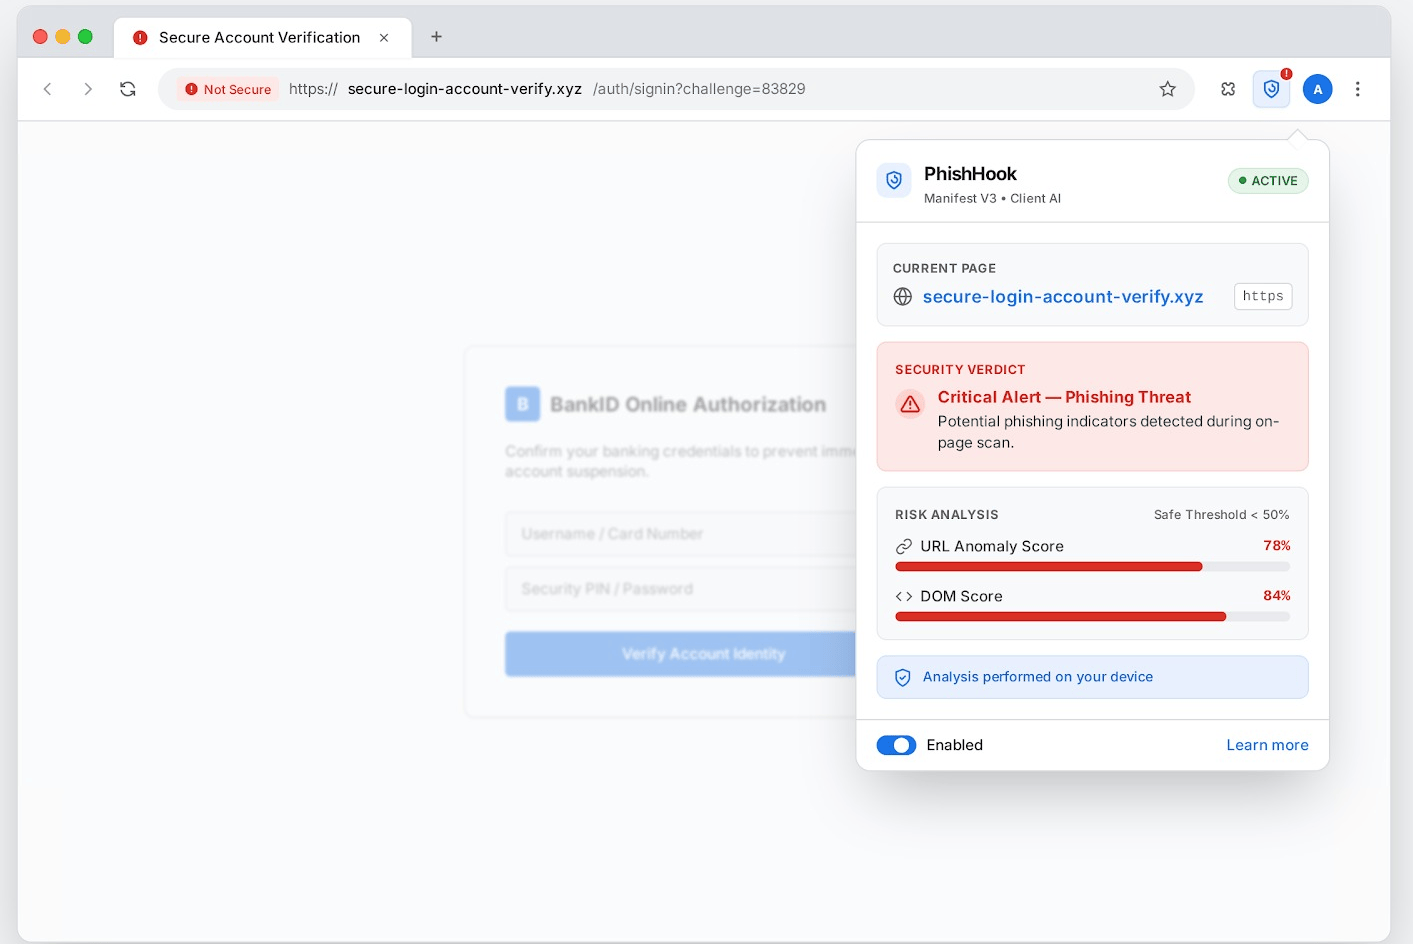
\includegraphics[width=0.9\textwidth]{Figures/gui_popup.png}
    \caption{Extension popup showing status and current verdict.}
    \label{fig:gui-popup}
\end{figure}

\subsection{Web Phishing Warning Banner}
The banner appears at the top of a web page when the fused risk score exceeds the deployed threshold. It states that the page is suspected of phishing and is dismissible.

\begin{figure}[H]
    \centering
    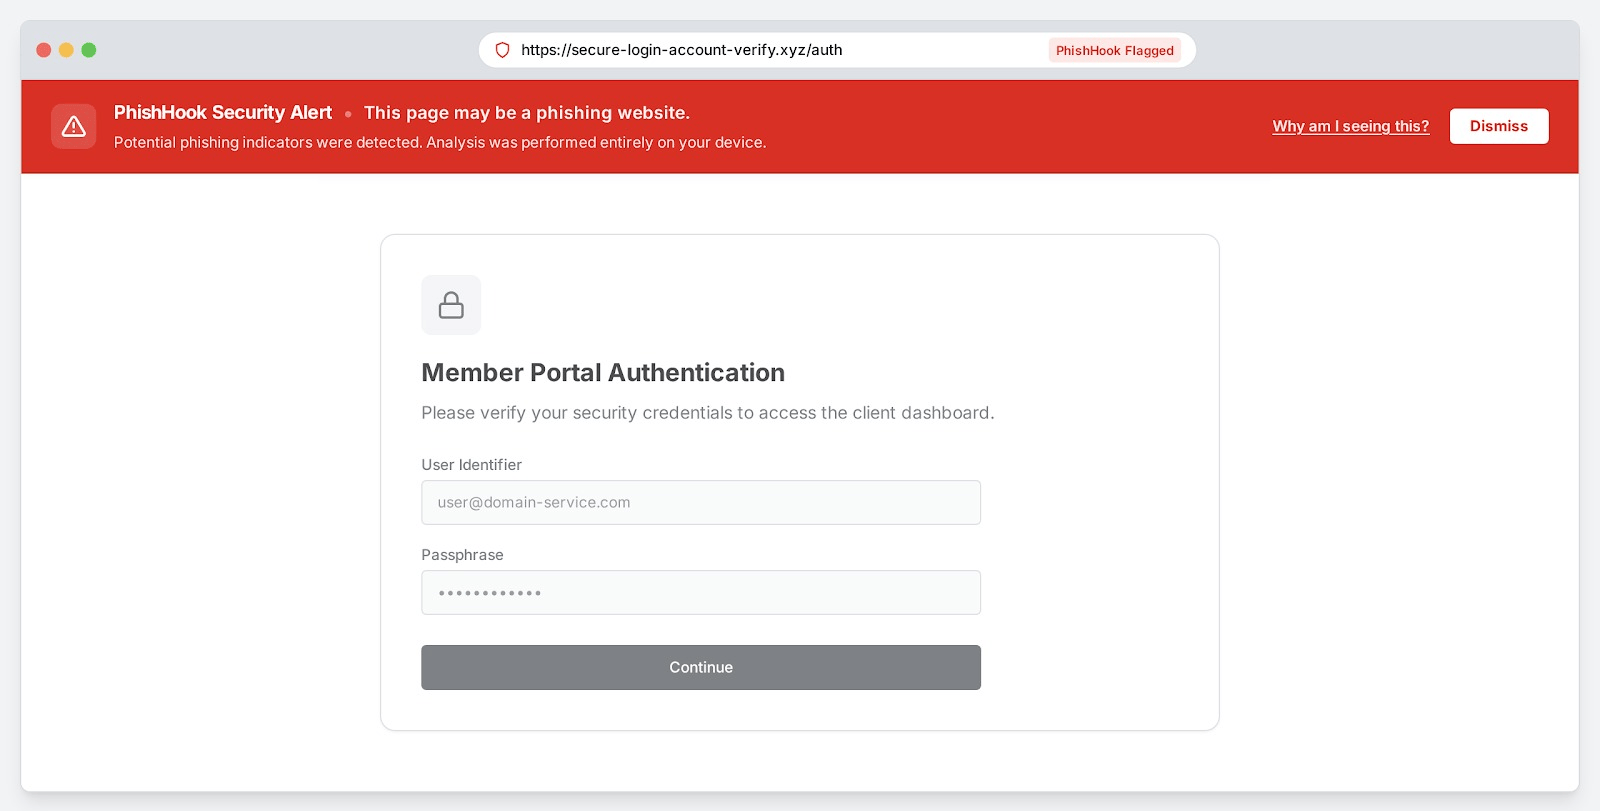
\includegraphics[width=0.9\textwidth]{Figures/gui_banner_web.png}
    \caption{Phishing warning banner on a web page.}
    \label{fig:gui-banner-web}
\end{figure}

\subsection{Form Submission Warning}
The form submission warning appears when a user attempts to submit a form on a page flagged as suspicious. It is worded more strongly than the passive banner.

\begin{figure}[H]
    \centering
    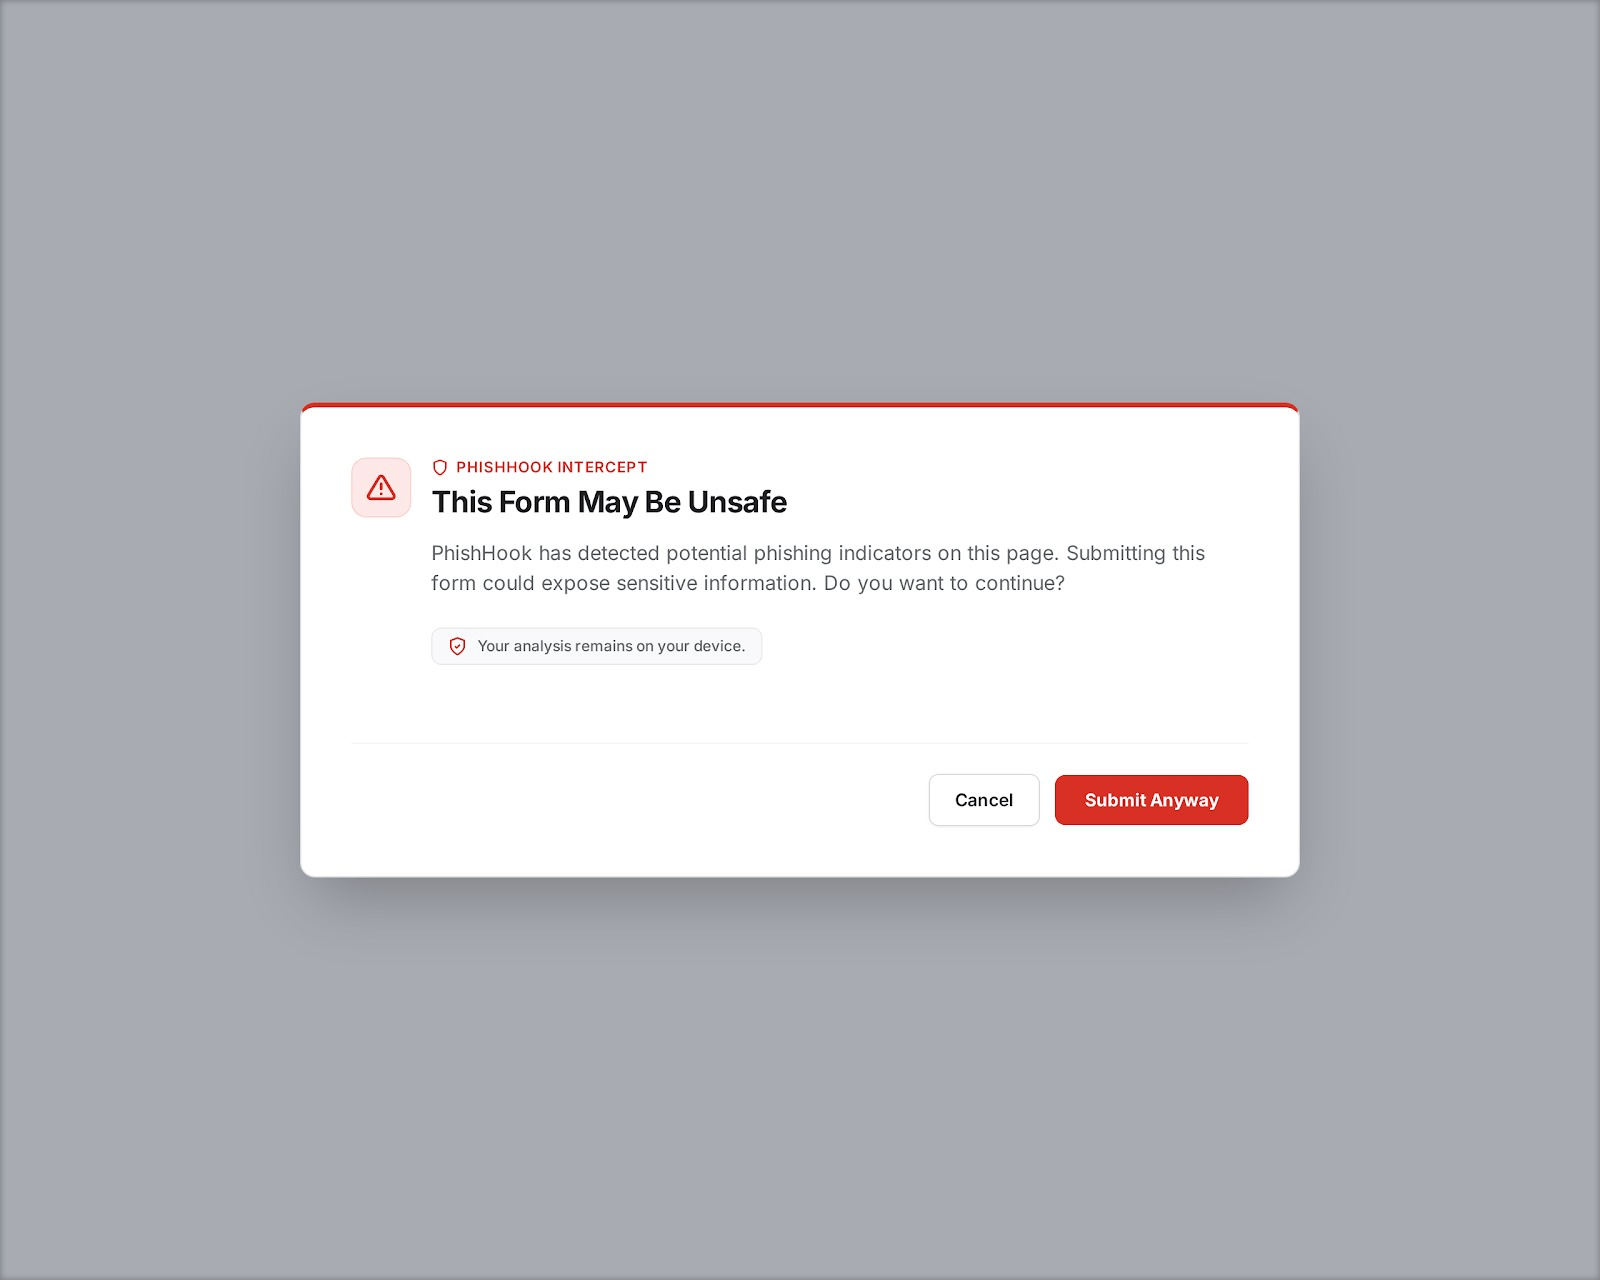
\includegraphics[width=0.9\textwidth]{Figures/gui_banner_form.png}
    \caption{Form submission warning.}
    \label{fig:gui-banner-form}
\end{figure}

\subsection{Email Phishing Warning Banner}
The email warning appears inside Gmail or Outlook web when the distilled BiLSTM student flags a message as phishing.

\begin{figure}[H]
    \centering
    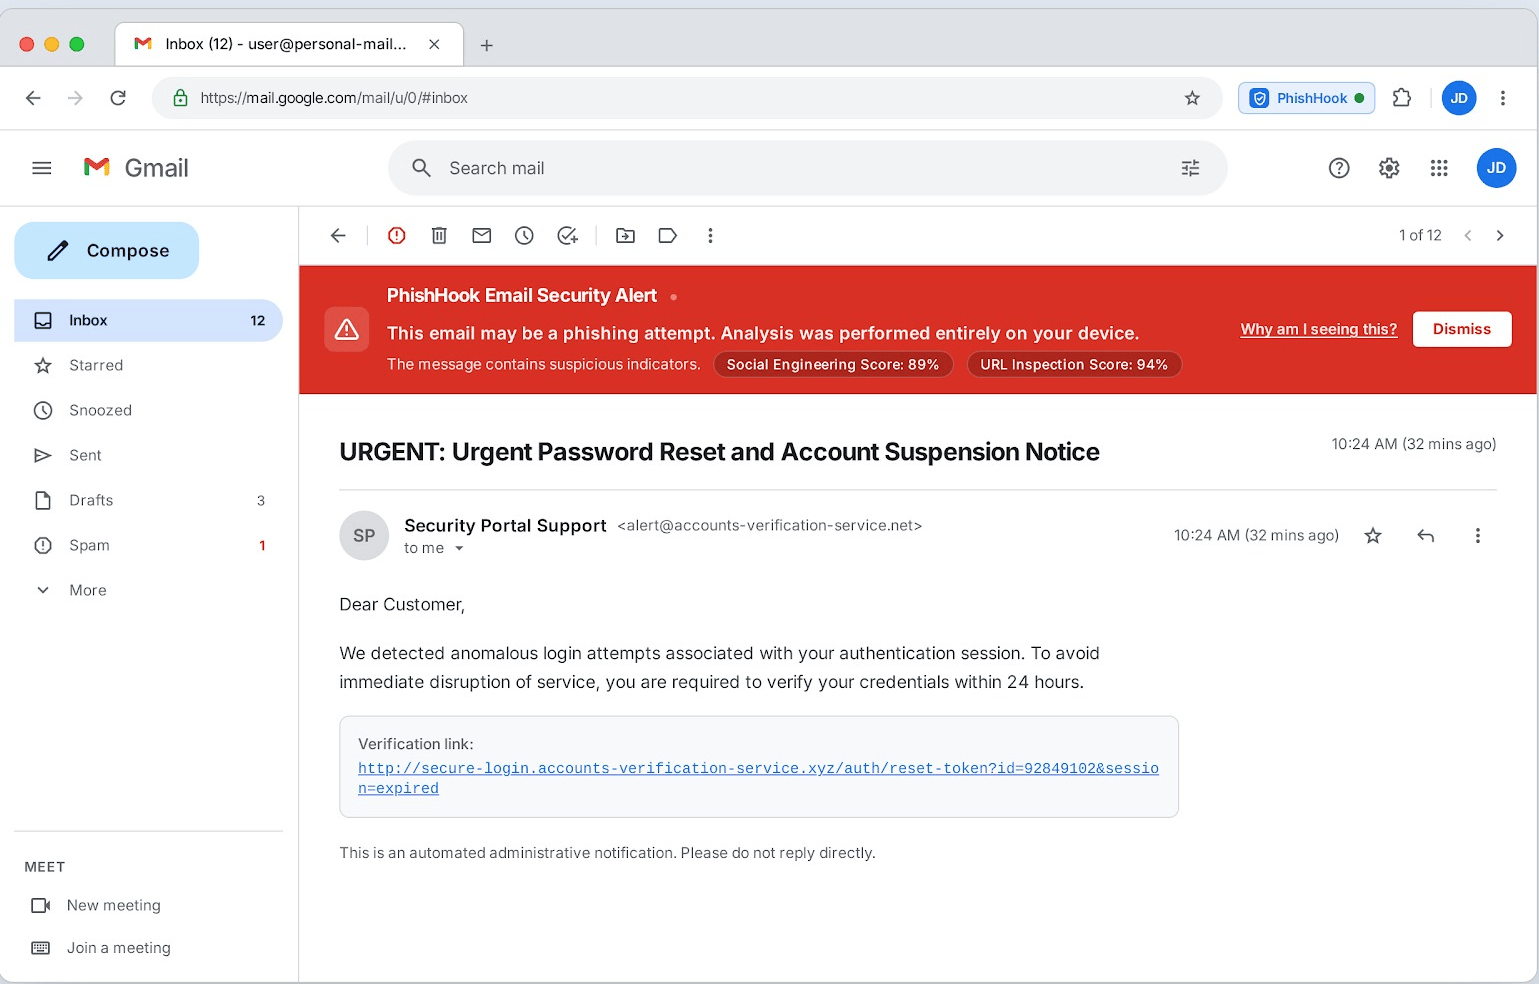
\includegraphics[width=0.9\textwidth]{Figures/gui_banner_email.png}
    \caption{Email phishing warning banner in webmail.}
    \label{fig:gui-banner-email}
\end{figure}

\section{Risk Analysis}
As PhishHook uses machine learning to detect phishing websites and emails, it is important to identify potential technical, security, privacy, and operational risks, that are discuss below.

\subsection{Technical Risks}
The effectiveness of PhishHook depends on the quality and diversity of the datasets used to train and evaluate its phishing detection models. Biased, outdated, or insufficient datasets may cause poor generalisation and increase false-positive or false-negative rates. The datasets come from public sources including PhishPedia, PhishTank, Tranco, and the merged MeAJOR email corpus, and email datasets in particular may contain personal information even after cleaning, which raises data-leakage concerns during training. 

\subsection{Model Performance Risks}
PhishHook combines URL analysis, webpage content classification, and email phishing detection. Errors in individual models or their fusion mechanism may lead to incorrect phishing verdicts. Moreover, a model that performs well on a test dataset may not achieve the same performance on previously unseen phishing attacks.

\subsection{Browser Compatibility and Resource Risks}
Running machine learning models entirely within a Chrome extension may introduce limitations related to model size, memory consumption, inference latency, and browser runtime compatibility. Large models may slow down webpage analysis or negatively affect the browsing experience.

\subsection{Security Risks}
As a browser extension, PhishHook requires access to webpage information to identify phishing indicators. Excessive permissions or insecure handling of extracted content could expose users to additional security risks. Malicious or manipulated webpages may also attempt to interfere with content extraction or trigger excessive analysis.

\subsection{Adversarial Evasion Risks}
Because PhishHook ships its models inside the extension package, the models are available to any user and therefore to any attacker. An adversary can inspect the model and design a phishing page specifically crafted to be classified as benign. This risk is inherent to any locally deployed detector and cannot be eliminated. 

\subsection{Ethical and Privacy Risks}
PhishHook analyses potentially sensitive information, including webpage content, URLs, and email messages. Improper handling or unintended storage of this information could compromise user privacy.

\subsection{Operational and Maintenance Risks}
Changes in Chrome, Manifest V3 APIs, webmail interfaces, or model runtime dependencies may affect the functionality of PhishHook. Similarly, changes in phishing techniques may reduce the effectiveness of existing detection models over time.

\section{Conclusion}
This chapter describes PhishHook's functional and non-functional requirements and the hardware and software needed to develop and deploy the extension. It provides a comprehensive road map by presenting the list of features, functional and non-functional requirements, quality attributes, assumptions, use cases, and the graphical user interface. The chapter emphasises the importance of privacy, security, reliability, efficiency, portability, and usability, which together ensure that the extension performs accurate ondevice phishing detection without transmitting any user data off the device. Additionally, user assumptions, and a comprehensive risk analysis covering technical, security, privacy, operational, and adversarial concerns are also explained. 



\chapter{Proposed Approach and Methodology}
\label{ch:methodology}

This chapter describes the methodology used to build and evaluate PhishHook, a client-side phishing detector for Chromium browsers that extends PhishLang \cite{phishlang2026}. It first presents the overall framework and briefly states what PhishHook keeps from PhishLang and what it changes. It then presents the data sources and how the data is prepared. The central part of the chapter explains how the URL and the rendered page are acquired and parsed on the user's device, including how JavaScript-generated content and dynamic page changes are handled. The chapter then details the algorithms behind each module, an unsupervised URL anomaly detector, a supervised page-content classifier, a fusion model, and a distilled email classifier. It also defines the model comparisons, evaluation metrics, statistical tests, resource measurement protocol and adversarial tests used to judge the design. (Chapter~\ref{ch:design}).

\section{Overview of the Proposed Framework}
\label{sec:framework}

PhishHook is a framework made of an input acquisition stage followed by independent detection modules whose outputs are combined into one verdict. It runs entirely inside a Manifest V3 browser extension. It uses only two local sources: the URL string of the page the user has loaded and the already-rendered Document Object Model (DOM) of that page. It never fetches pages itself, performs no WHOIS, DNS, domain-age, search-index or reputation lookups, and transmits nothing off the device.

PhishHook extends PhishLang \cite{phishlang2026}, a fully client-side phishing detection framework that uses MobileBERT over a compact, structured representation of a page's actionable elements. PhishHook keeps that fully-local, transformer-based page-classification core and adds five things that PhishLang does not do. First, the URL is handled by a separate unsupervised module, and the URL itself is excluded from the DOM model's input so that the two modules stay complementary. Second, the two scores are combined by a small calibrated fusion model, trained on scores that are out of sample for the DOM model. Third, dynamic changes to the page after load are observed, and significant changes trigger re-analysis. Fourth, results are reported at low false-positive rates, at stated base rates, and on source-disjoint and temporal test sets. Fifth, an email surface is added using knowledge distillation from a MobileBERT teacher into a compact BiLSTM student. Resource cost is measured inside the extension on both high-end and low-end hardware.

The framework has two user-facing surfaces:
\begin{itemize}
    \item \textbf{Web surface:} An unsupervised URL anomaly module and a supervised DOM classifier produce two scores, which a small fusion model combines into a single risk score.
    \item \textbf{Email surface:} A compact BiLSTM student, trained by distillation from a MobileBERT teacher, classifies the email shown in the webmail interface.
\end{itemize}

\begin{figure}[!ht]
\centering
\resizebox{\textwidth}{!}{%
\begin{tikzpicture}[
    node distance=0.5cm and 0.6cm,
    box/.style={draw, rounded corners, align=center, minimum height=1.0cm, text width=2.3cm, font=\footnotesize, fill=blue!5},
    off/.style={draw, dashed, rounded corners, align=center, minimum height=1.0cm, text width=5.4cm, font=\footnotesize, fill=gray!10},
    arr/.style={-{Latex}}
]
% web row
\node[box] (page) {Loaded web page};
\node[box, right=of page] (extract) {URL parser and DOM parser};
\node[box, right=of extract, yshift=0.9cm] (url) {URL anomaly module};
\node[box, right=of extract, yshift=-0.9cm] (dom) {DOM classifier (MobileBERT, int8)};
\node[box, right=of url, yshift=-0.9cm] (fuse) {Fusion (logistic regression)};
\node[box, right=of fuse] (verdict) {Verdict and warning};
\draw[arr] (page) -- (extract);
\draw[arr] (extract) -- (url);
\draw[arr] (extract) -- (dom);
\draw[arr] (url) -- (fuse);
\draw[arr] (dom) -- (fuse);
\draw[arr] (fuse) -- (verdict);
\draw[arr, dashed] (extract.south) |- ++(0,-1.9cm) -| (verdict.south) node[pos=0.25, below, font=\scriptsize]{URL-only fallback if DOM unavailable};
% email row
\node[box, below=3.2cm of page] (mail) {Webmail page};
\node[box, right=of mail] (mparse) {Email parser};
\node[box, right=of mparse] (student) {BiLSTM student (distilled)};
\node[box, right=of student] (mverdict) {Email verdict};
\draw[arr] (mail) -- (mparse);
\draw[arr] (mparse) -- (student);
\draw[arr] (student) -- (mverdict);
% offline
\node[off, below=0.9cm of student] (offline) {Offline only (not deployed): MobileBERT teacher, reference baselines};
\draw[arr, dashed] (offline.north) -- (student.south) node[midway, right, font=\scriptsize]{distillation};
\end{tikzpicture}%
}
\caption{Overview of the PhishHook framework. Solid boxes run inside the browser extension; the dashed box is used only during training and comparison.}
\label{fig:framework}
\end{figure}

\begin{table}[!ht]
\centering
\caption{Deployed and offline-only components.}
\label{tab:components}
\begin{tabularx}{\textwidth}{|>{\raggedright\arraybackslash}X|>{\raggedright\arraybackslash}X|>{\raggedright\arraybackslash}X|}
\hline
\textbf{Component} & \textbf{Role} & \textbf{Deployed in extension?} \\
\hline
URL anomaly model (autoencoder or Isolation Forest) & Scores the URL string; trained on benign URLs only & Yes (the selected one) \\
\hline
DOM MobileBERT (int8) & Classifies parsed page text; the URL is excluded from its input & Yes \\
\hline
Fusion model & Combines the two web scores & Yes \\
\hline
BiLSTM student & Classifies emails visible in the webmail interface & Yes \\
\hline
MobileBERT teacher (email) & Produces soft labels for distillation & No (training only) \\
\hline
Reference baselines (K-Means/IF URL baseline, MobileBERT on URL strings, LightGBM on DOM features) & Measure what a simpler or supervised method achieves & No (comparison only) \\
\hline
\end{tabularx}
\end{table}

\section{Datasets and Data Preparation}
\label{sec:data}

\subsection{Data Sources}
\begin{itemize}
    \item \textbf{PhishPedia} \cite{phishpedia2021}: A labelled web phishing dataset that pairs phishing and benign pages with their URLs and HTML. We use it to train the supervised page-content model and to run in-distribution tests.
    \item \textbf{PhishTank}: A community-driven phishing feed. We crawl the reported phishing URLs to collect both the URL and the rendered DOM, and use it as a source-disjoint and temporal test set.
    \item \textbf{Benign URL sources}: Deeper-ranked domains from the Tranco list, combined with real URL paths taken from public crawl indexes or pulled from links on benign pages. We use these to train the unsupervised URL module and to measure false-positive rates.
    \item \textbf{PhiUSIIL}: A phishing URL dataset with 134,850 legitimate and 100,945 phishing URLs, each described by 56 features extracted from the URL and the page source. It is the main dataset for training and evaluating the unsupervised URL anomaly module.
    \item \textbf{MeAJOR corpus} \cite{meajor2025}: A merged, multi-source email phishing dataset that we use for the email study.
\end{itemize}

\subsection{Data Roles and Separation Principles}
\label{sec:roles}

The actual size of the splits is predetermined in the experimental plan. Regardless of the eventual division, the following roles and rules will be in effect.

\begin{itemize}
    \item \textbf{Training Data:} Used to train the model and learn its weights. It provides the examples from which the model learns relevant patterns and relationships during the training process.

    \item \textbf{Tuning Data:} Used to adjust hyperparameters and determine when training should stop. It helps monitor model performance during development and supports decisions about the final training configuration.

    \item \textbf{Calibration and Fusion Data:} Kept separate from DOM model training to ensure that the scores are generated on unseen data. It is used to calibrate the DOM model, train the fusion model, and select decision thresholds. This separation helps prevent the calibration process from benefiting unfairly from samples already seen during model training.

    \item \textbf{Test Data:} Reserved for the final evaluation of the system. It includes an in-distribution test set, a source-disjoint and temporal test set, and a small collection of pages captured during real browsing sessions. These subsets provide different perspectives on system performance under both familiar and less familiar conditions.

    \item \textbf{Unsupervised URL Data:} The unsupervised URL model is trained using benign URLs only. Phishing URLs are excluded from training. A separate benign validation set is used to establish reference scores for percentile ranking and threshold selection. This allows unusual URL patterns to be identified without using phishing labels during training.

    \item \textbf{Leakage Prevention:} Samples and their near-duplicates, including those from the same domain or phishing campaign, are kept separate across data splits. Test data is never used for model selection, hyperparameter tuning, threshold selection, or calibration. This ensures that the final evaluation provides a fair assessment of the system's ability to generalize to unseen samples.
\end{itemize}

\subsection{PhishTank Collection Protocol}

Collecting live phishing pages can involve security risks and data quality issues. To avoid these problems, a consistent procedure is followed during data collection.

\begin{itemize}
    \item \textbf{Safe Environment:} All pages are accessed through an isolated and disposable browser environment rather than a personal computer or account.

    \item \textbf{No Personal Information:} No login credentials or personal information are entered on any phishing page during collection.

    \item \textbf{Submission Time:} The submission timestamp provided by the feed is recorded to maintain the correct time order of the collected pages.

    \item \textbf{Page Rendering:} Each page is opened in a real browser to allow JavaScript to execute. The resulting DOM and its corresponding URL are then saved.

    \item \textbf{Page Filtering:} Pages that are no longer active, parked, empty, showing errors, or clearly cloaked are excluded. The number of excluded pages is also recorded.

    \item \textbf{Label Verification:} Since community-based feeds may contain incorrect labels, a random sample of collected pages is manually checked to estimate the possible labeling error.
\end{itemize}

\subsection{Benign URL Set and Popularity Bias}

An anomaly detector trained only on benign URLs may incorrectly identify less popular domains or URLs containing paths as suspicious. To reduce this problem, the following measures are included:

\begin{itemize}
    \item \textbf{Training Data Diversity:} The benign training set includes domains beyond the most popular rankings. It also contains URLs with actual paths and query parameters.

    \item \textbf{Separate Evaluation:} The evaluation is divided into homepage-only URLs and URLs containing paths or queries. This helps identify whether the model is relying too heavily on URL structure.

    \item \textbf{Ablation Study:} Paths and query parameters are removed from all URLs before scoring to examine how much the model's performance depends on these features.
\end{itemize}

If a suitable source of less popular benign URLs is not available, this limitation will be clearly mentioned in the report.

\subsection{Cleaning and Deduplication}
Duplicates are removed at the URL, domain and campaign level. The benign URL training data is deduplicated against all other benign data used anywhere in the study, so that no URL used to train the unsupervised model is later used to measure its false-positive rate.

\subsection{Mapping Emails to the Webmail View}

MeAJOR stores emails in their original form, while the extension can only access the information visible on a webmail page. To keep the training data consistent with what the extension can actually observe, each email is converted into a webmail-style representation before training.

\begin{itemize}
    \item \textbf{Subject:} The subject line is kept as plain text.

    \item \textbf{Sender:} Only the sender's display name and email address visible on the screen are included, without relying on hover information.

    \item \textbf{Body:} The HTML content is converted into visible text, with scripts, styles, tracking pixels, and hidden elements removed.

    \item \textbf{Links:} Both the displayed link text and the destination host are retained.

    \item \textbf{Attachments:} Only the file names visible in the webmail interface are included.

    \item \textbf{Headers:} Email headers are completely excluded so that training does not use information that the extension cannot access.
\end{itemize}

\subsection{Required Benign Sample Size for False-Positive Estimates}
\label{sec:fpr-size}
The evaluation focuses on low false-positive rates, which need many benign samples to estimate reliably. To estimate a false-positive rate $p$ with a relative standard error $r$, about
\begin{equation}
n \;\ge\; \frac{1-p}{p\, r^{2}}
\end{equation}
benign samples are needed. For $r = 0.2$ this gives about 2{,}475 samples for $p = 1\%$ and about 24{,}975 samples for $p = 0.1\%$.

\section{Input Acquisition and Parsing}
\label{sec:input-acquisition}

This section explains how the extension obtains the URL and the page content on the user's device and turns them into model inputs. The same procedures are used to prepare the training data.

\subsection{What Is Read and When}

\begin{itemize}
    \item \textbf{URL:} The URL of the main page is obtained from the browser's navigation information once the navigation has been completed.

    \item \textbf{Rendered DOM:} The content script collects the rendered DOM after the page has finished loading and its content is stable.
\end{itemize}

\subsection{URL Acquisition and Parsing}
\label{sec:url-parsing}

The original URL is preserved exactly as reported by the browser for the unsupervised character-level model. A separate parsed copy is prepared for the feature-based model using the following steps.

\begin{itemize}
    \item \textbf{URL Components:} The URL is divided into its main parts, including the scheme, host, port, path, query, and fragment.

    \item \textbf{Host-Based Features:} The number of subdomain levels, host labels, and hyphens is counted. The parser also checks whether the host is an IP address.

    \item \textbf{Internationalised Domains:} Domain names are decoded from their punycode representation, and the presence of punycode is recorded as a separate feature.

    \item \textbf{Path and Query Analysis:} The path is divided into individual segments, while the query string is separated into parameters. The number of segments and parameters is also recorded.

    \item \textbf{Percent Encoding:} Percent-encoded characters are identified, and their decoded forms are used for statistical analysis. The original URL is retained for the character-level model.

    \item \textbf{Statistical Features:} Length, digit ratio, and character entropy are calculated separately for the host, path, and query. The longest consecutive sequence of digits is also recorded.

    \item \textbf{Top-Level Domain:} The frequency rank of the top-level domain is obtained from a reference table built using benign training data.

    \item \textbf{Scheme Exclusion:} The scheme (\texttt{http} or \texttt{https}) is excluded from the feature set because it may reflect when a dataset was collected rather than whether a URL is malicious.
\end{itemize}

\subsection{Rendered DOM Acquisition}
\label{sec:dom-acquisition}

The content script collects information from the live, rendered DOM rather than the original HTML source downloaded by the browser. This allows the system to work with the page as it appears after scripts and other dynamic changes have taken place.

\begin{itemize}
    \item \textbf{Top-level document:} The complete rendered DOM of the main page is read, including elements added, moved, or changed by scripts after the page initially loads.

    \item \textbf{Same-origin frames:} Frames that share the same origin as the main page are also read, and their content is included as part of the main page.

    \item \textbf{Cross-origin frames:} The browser restricts access to frames belonging to a different origin. Therefore, only the frame's source host is recorded. This is a known limitation, as phishing forms placed inside such frames cannot be accessed by the parser.

    \item \textbf{Shadow DOM:} Open shadow roots are traversed, and their content is included in the extracted text. Closed shadow roots are not accessible to external scripts. As a result, any content placed inside them remains unavailable to the parser.
\end{itemize}

\subsection{DOM Parsing and Serialisation Algorithm}
\label{sec:dom-parsing}
MobileBERT is not supplied with the raw DOM or raw HTML by the parser. Rather, it obtains a small and organized model of elements on a page that can be acted on, in the style of PhishLang \cite{phishlang2026}. The process is as follows.

\begin{itemize}
    \item \textbf{Traverse the rendered DOM:} The parser moves through the DOM in a depth-first manner, with a limit on the number of nodes it visits. This prevents very large pages from slowing down or freezing the browser.

    \item \textbf{Skip non-content nodes:} Scripts, styles, comments, and template elements are removed because they do not contain information that is directly visible to the user.

    \item \textbf{Skip invisible nodes:} Elements that are hidden, not displayed, have zero size, or are positioned far outside the visible area are excluded. This is important because attackers may use hidden text or form fields to mislead the model with content that users cannot actually see. By focusing on visible elements, the parser reduces the risk of this type of manipulation.

    \item \textbf{Extract the feature groups:} The parser collects the feature groups listed in Table~\ref{tab:dom-groups} from the remaining visible elements. Each group represents a type of page element that may contain useful information for detecting phishing, following the feature-extraction approach used by PhishLang.

    \item \textbf{Normalise the extracted text:} Repeated spaces are reduced, control characters are removed, and exact duplicate entries are eliminated to keep the extracted content clean.

    \item \textbf{Serialise each group:} Each feature group is converted into a short text segment with a label, such as \texttt{TITLE: ...}, \texttt{FORMS: ...}, or \texttt{ANCHORS: ...}. These segments are then combined in a fixed priority order.
\end{itemize}

The parser uses extracted features instead of passing the entire raw DOM to the model for several reasons. First, a complete DOM can be too large to fit within MobileBERT's 512-token limit. Simply cutting off the extra content could remove important details that help identify a phishing page. Second, selecting specific feature groups ensures that important elements, particularly the page title and login form, are included in the model input even when the page contains a large amount of content. Finally, this approach removes unnecessary styling, layout information, and repeated page content that do not contribute to phishing detection. As a result, the model receives a smaller and more focused representation of the page.

\begin{table}[!ht]
\centering
\caption{Element groups extracted from the rendered DOM, in priority order.}
\label{tab:dom-groups}
\begin{tabularx}{\textwidth}{|c|>{\raggedright\arraybackslash}X|>{\raggedright\arraybackslash}X|}
\hline
\textbf{Priority} & \textbf{Group} & \textbf{What is extracted} \\
\hline
1 & Title and headings & The page title and the main visible headings \\
\hline
2 & Brand cues & Alternative text and labels of logos and images \\
\hline
3 & Forms and inputs & Field labels, placeholders, field names and types, button text \\
\hline
4 & Anchors (HREFs) & Visible link text and the destination host only; repeated hosts counted once \\
\hline
5 & Scripts and iFrames & The presence of these elements and the source hosts of frames \\
\hline
6 & Footer and helper links & Policy, help and account links \\
\hline
7 & Visible body text & Remaining visible text, deduplicated, in reading order \\
\hline
\end{tabularx}
\end{table}

The URL of the page is deliberately not part of this representation. The URL module sees only the URL and the DOM module sees only the page content, so the two modules remain complementary and the fusion has two independent signals to combine. Including the URL in the DOM model's input would cause the two modules to overlap, and the fusion would add no value.

\subsection{Token Budget and Truncation}
\label{sec:token-budget}

MobileBERT has a maximum input limit of 512 tokens. To stay within this limit while retaining the most useful page information, the serialised representation is reduced using the following rules.

\begin{itemize}
    \item \textbf{Per-group item caps:} A maximum number of items is set for each of the seven groups listed in Table~\ref{tab:dom-groups}. This prevents a single group with many elements from taking up most of the available token space.

    \item \textbf{Priority-ordered concatenation:} The groups are combined according to the priority order shown in Table~\ref{tab:dom-groups}. The page title, brand cues, forms, and inputs are placed first, while visible body text is included towards the end.

    \item \textbf{Truncation at the tail:} If the combined representation still exceeds the 512-token limit, content is removed from the end. Since the groups considered less informative are placed last, this helps retain the information most relevant to phishing detection.

    \item \textbf{No page-size shortcut:} Page-size information is not provided to the model. Combined with the per-group item caps, this prevents the model from relying on page size as a shortcut when making predictions.
\end{itemize}

Since the title, brand cues, forms, and inputs are placed at the beginning of the representation, they are retained even when truncation is required. The frequency of truncation and the groups most commonly affected are also measured and reported.

\subsection{Handling JavaScript-Rendered and Dynamic Content}
\label{sec:js-dynamic}

Phishing pages often use JavaScript to display content or make changes to the page after it has initially loaded. To capture these changes, the extension handles dynamic content using the following steps.

\begin{itemize}
    \item \textbf{Read after rendering:} The content is extracted from the live DOM after the page's load event, rather than from the initial HTML.

    \item \textbf{Wait for the DOM to settle:} After the load event, the extension waits for a short period during which no relevant changes occur. A maximum waiting time is also set to avoid unnecessary delays.

    \item \textbf{Observe changes:} A mutation observer monitors the page for newly added or removed elements and changes to existing attributes after the initial analysis.

    \item \textbf{Single-page applications:} If the page address changes without a full reload, the extension treats it as a new page and performs the analysis again from the beginning.

    \item \textbf{Time-bounded work:} DOM traversal is divided into smaller tasks and carried out during the page's idle time to reduce interference with normal browsing.
\end{itemize}

\subsection{Dynamic Monitoring and Re-Trigger Policy}
\label{sec:dynamic-trigger}

Analysing every change made to a page would require unnecessary processing. Therefore, the extension only starts a new analysis when a change is considered significant. Six types of changes are monitored. First, the appearance or visibility of a password field or a new form is treated as significant, since collecting login credentials is a common goal of phishing pages. Second, a noticeable change in the number of visible input fields may indicate that a login form has been added after the page loads. Third, changes to the page title or brand-cue elements are monitored because they may indicate a change in the page's identity. Fourth, the addition of a frame with a new source is considered important, as it may introduce content from another origin. Fifth, replacing a large portion of the visible page content may indicate that the page has been rebuilt. Finally, a client-side route change is treated as a new event because it may display a different page without requiring a full reload.

The re-analysis process follows these steps:

\begin{itemize}
    \item \textbf{Detect a change:} The mutation observer reports a change detected on the page.

    \item \textbf{Check its significance:} The extension checks whether the change matches one of the six significant event types. Other changes are ignored to avoid unnecessary analysis.

    \item \textbf{Apply debouncing:} Multiple events are grouped together, and analysis begins only after the page has remained unchanged for a short interval.

    \item \textbf{Limit repeated analysis:} A cool-down period and a maximum number of analyses per page are used to control processing costs.

    \item \textbf{Handle pending requests:} If an analysis is already in progress, the latest request replaces any older request waiting to be processed.

    \item \textbf{Update the verdict:} Once the new analysis is complete, the previous verdict is updated. If the page changes from benign to suspicious, the extension displays a warning at that point.
\end{itemize}

\subsection{Parsing Webmail Content}
\label{sec:email-parsing}

Email content is extracted directly from the webmail page's DOM using a separate adapter for each supported client, namely Gmail and Outlook web. Each adapter identifies the currently open email and collects the same fields used in the training data mapping. For every link, the extension also checks whether the host displayed in the link text matches the actual destination host. The extension does not open links or retrieve their destinations, so each link is assessed using its address and the surrounding context.

\subsection{Training--Deployment Parity}
\label{sec:parity}

The same parser used by the extension is also applied to the training pages to keep the processing consistent across both stages. When a dataset contains only downloaded HTML, the page is first opened in a real browser so that its scripts can run and generate the rendered DOM. The resulting DOM is then passed through the parser. In addition, a small collection of pages captured during actual browsing sessions is included as a separate test set to examine how the system performs on real-world pages.

\section{Module A: Unsupervised URL Anomaly Detection}
\label{sec:url-module}

This module focuses on identifying unusual URLs by learning the patterns found in benign web addresses. Unlike supervised approaches, it does not use phishing URLs during training. Instead, it learns the characteristics of normal URLs and assigns higher anomaly scores to URLs that differ from these learned patterns. Three candidate approaches are considered and compared to determine their effectiveness.

\subsection{Problem Formulation}

Let $u$ represent a URL. The module assigns an anomaly score $s(u)$, where a higher score indicates that the URL differs more from the benign URLs used during training. A URL is marked as anomalous when its score exceeds a threshold $\tau$. This threshold is selected using benign validation data to achieve the target false-positive rates of 1\% and 0.1\%.

\subsection{Candidate 1: Character-Level Autoencoder}

\paragraph{Preprocessing.} Each character is converted into an index from a fixed vocabulary. All URLs are then adjusted to a fixed length $L$ by either truncating longer URLs or padding shorter ones. A mask is used to identify the padded positions so they are excluded from the calculations.

\paragraph{Architecture.} The model uses a convolutional encoder to convert the character sequence into a compact latent representation. A decoder then reconstructs the sequence by predicting a probability distribution over the character vocabulary at each position.

\paragraph{Training Objective.} Let $c_i$ represent the actual character at position $i$, $p_i(c_i)$ its predicted probability, and $M$ the set of positions that do not contain padding. The reconstruction loss is also used as the anomaly score:

\begin{equation}
s(u) \;=\; -\frac{1}{|M|}\sum_{i\in M} \log p_i(c_i).
\end{equation}

The model is trained to minimise this loss across the benign training URLs. URLs that are less familiar to the model are expected to produce higher reconstruction errors.

\paragraph{Length Sensitivity.} The reconstruction error can vary depending on URL length and character diversity. To account for this, performance is also evaluated separately across different URL length groups.

\subsection{Candidate 2: Isolation Forest on Lexical Features}

\paragraph{Features.} The model uses the lexical features described in Section~\ref{sec:url-parsing}. These include separate statistics for the host, path, and query, along with subdomain depth, path depth, query parameter count, hyphen and dot counts in the host, longest digit sequence, punycode and percent-encoding flags, and the top-level domain rank.

\paragraph{Algorithm.} Isolation Forest identifies unusual samples by measuring how easily they can be separated from the rest of the data. For a sample $x$ and a training sample size $n$, the anomaly score is calculated as:

\begin{equation}
s(x,n) \;=\; 2^{-\,E[h(x)]/c(n)},
\end{equation}

where $h(x)$ represents the number of splits required to isolate $x$, and $E[h(x)]$ is the average path length across all trees. The term $c(n)$ represents the expected path length of an unsuccessful search in a binary search tree containing $n$ points. Scores closer to 1 indicate a higher likelihood of the sample being anomalous.

\paragraph{Feature Justification.} To examine the contribution of individual feature groups, the model is evaluated after removing one group at a time. The groups include host, path, query, top-level domain, and encoding features. The resulting changes in performance are recorded to determine which groups contribute most to anomaly detection.

\subsection{Candidate 3: K-Means Distance Baseline}

As an additional baseline, a K-Means model is trained using the same benign lexical features. Each URL is assigned an anomaly score based on its distance from the nearest cluster centroid. This approach provides a simple reference for comparing the performance of the two main candidates against a basic clustering method. The K-Means model is included only for comparison and is not part of the deployed system.

\subsection{Testing the Unsupervised Approach}
\begin{itemize}
    \item \textbf{Separation test:} Are there significantly different distributions of scores for benign and phishing URLs in the validation data set?
    \item \textbf{Training-set composition:} Compare models trained on top-ranked benign domains only with models trained on deeper-ranked benign URLs.
    \item \textbf{Training-set size:} Measure performance as the amount of benign training data grows.
    \item \textbf{Path and query ablation:} Remove path and query from all URLs and compare.
    \item \textbf{Length analysis:} Report scores and detection by URL length band.
    \item \textbf{Shift robustness:} Evaluate on the source-disjoint and temporal test sets.
\end{itemize}

\subsection{Supervised Reference Model and URL Comparison}
\label{sec:url-comparison}
To see what the unsupervised module can do well and where it falls short, it is compared with a supervised model on the same task using the same test data. MobileBERT is fine-tuned on the raw URL text to tell phishing and benign URLs apart. This supervised model is used only for comparison and is never deployed in the extension. The deployed DOM classifier is a different model that looks at page content and never sees the URL.

Four URL models are compared in total. The Isolation Forest is trained only on benign URLs and is an unsupervised candidate for deployment. The K-Means distance baseline is also trained only on benign URLs and is an unsupervised reference; it shows whether the Isolation Forest is actually better than a simpler method and can be deployed if it outperforms the Isolation Forest. The character-level autoencoder is also trained only on benign URLs and is another unsupervised reference. The MobileBERT on URL strings is trained on labelled URLs and is the supervised reference; it is never deployed.

The comparison is interpreted fairly. The supervised model is given phishing labels during training, so it is expected to do well on data similar to its training set. The real question is how large the gap is between the supervised model and the unsupervised models at a low false-positive rate, whether that gap grows when the data comes from a different source or a later time, and how much the models cost in size and speed.

\subsection{Percentile-Rank Transformation}
Raw anomaly scores of different models are not comparable. For fusion, the score of the selected model is converted to a percentile rank among benign validation scores $s_1,\dots,s_m$:
\begin{equation}
r(s) \;=\; \frac{1}{m}\,\bigl|\{\,j : s_j \le s\,\}\bigr| .
\end{equation}
About one thousand reference quantiles are stored in the extension.

% ============================================================
\section{Module B: Supervised DOM Classification}
\label{sec:dom-module}

\subsection{Input and Model}
The model receives the serialised representation of Section~\ref{sec:dom-parsing}, built from the seven feature groups of Table~\ref{tab:dom-groups} and trimmed to the token budget of Section~\ref{sec:token-budget}. It outputs a phishing score for the page. MobileBERT is fine-tuned for binary classification.

\subsection{Baseline Model: LightGBM}
A gradient-boosted tree model is trained on engineered features extracted from the same seven DOM groups. The features include the number and types of form fields, the presence of a password field, the number of external link hosts, the number of iframes, the ratio of script nodes to total nodes, the number of brand-cue elements, the presence of specific keywords in the title, and page-length statistics. LightGBM is used only for comparison. It is not deployed and it is not part of the fusion pipeline.

\subsection{Fine-Tuning Procedure}
The model is fine-tuned on the training data, with hyperparameters and early stopping chosen on the tuning data. The search budget and random seeds are fixed in advance and reported.

\subsection{Quantisation, Export and Parity}

The trained model is exported into a portable format for deployment and converted to 8-bit integers through quantisation. A 16-bit version is also evaluated to examine the effect of an intermediate precision level. The accuracy, calibration, and model size are compared across the 32-bit, 16-bit, and 8-bit versions. A parity check is also performed to verify that the exported model produces results consistent with the original model within a specified tolerance.

\subsection{Model Comparison}

MobileBERT and LightGBM are evaluated using the same test sets and evaluation metrics to ensure a fair comparison. Bootstrap confidence intervals are calculated for each comparison to account for variation in the results. The evaluation examines whether a lightweight transformer provides better performance than a traditional tree-based model when both use the same DOM-derived features. Model size and inference latency are also considered to understand the cost of any performance improvement.

\subsection{Input Ablation}

To understand how different input components affect model performance, the model is trained and evaluated using several reduced input configurations. These include the full representation; title and brand cues only; title, brand cues, forms, and inputs; the same representation with anchors and scripts; visible body text only; and, as a control, the full representation with the URL added. Comparing these configurations helps identify which parts of the DOM representation contribute most to the model's performance.

\section{Module C: Fusion}
\label{sec:fusion}

\subsection{Model}
Fusion combines two inputs: the percentile rank $r$ of the URL anomaly score and the calibrated DOM score $z_{\mathrm{cal}}$. A logistic regression gives the combined probability:
\begin{equation}
P(\text{phishing}) \;=\; \sigma\!\left(w_1\, r + w_2\, z_{\mathrm{cal}} + b\right),
\end{equation}
where $w_1$, $w_2$ and $b$ are three numbers fitted on held-out data, and $\sigma$ is the logistic function that maps any value to a probability between 0 and 1. Training minimises the negative log-likelihood plus a small penalty $\lambda\,(w_1^2 + w_2^2)$ that keeps the weights from overfitting the small fitting set. Only three numbers and one threshold are needed in the extension.

\subsection{Leakage Control}
The fusion model is fitted only on data that was held out from the training of the DOM model, so the DOM scores it sees are genuinely unseen.

\subsection{Decision Threshold and Fallback}
The decision threshold is chosen on the same held-out data to hit target false-positive rates, not fixed at 0.5. If the page content is unavailable, the extension falls back to the URL score alone with its own threshold.

\subsection{Ablations and Complementarity}
Four configurations are compared at the stated base rates: URL only, DOM only, an OR rule, and the fused model. Complementarity is measured by the correlation between the URL score and the DOM score, and by the gain in detection from fusion.

% ============================================================
\section{Email Phishing Detection and Knowledge Distillation}
\label{sec:email}

\subsection{Models in the Study}
\begin{itemize}
    \item \textbf{MobileBERT teacher:} fine-tuned on the email training data.
    \item \textbf{Distilled BiLSTM student:} trained from the teacher's soft labels, the deployed email model.
\end{itemize}

\subsection{Teacher and Student}
The teacher is fine-tuned on the training emails in the webmail view, and its calibration is checked, because soft labels carry the teacher's confidence. The student is a bidirectional recurrent model with its own vocabulary and embeddings: an embedding layer, a bidirectional LSTM layer, a pooling step and an output layer. Because the teacher and the student use different tokenisations, distillation is done at the output level only.

\subsection{Quantisation, Export and Parity}

The model is exported in a portable format and quantised to 8-bit integers for deployment. A 16-bit version is also tested. The three versions are compared in terms of accuracy, calibration, and model size. A parity check ensures that the exported model produces results close to the original.

\subsection{Model Comparison}

MobileBERT and LightGBM are tested on the same datasets using the same evaluation metrics. Bootstrap confidence intervals are also calculated. The comparison examines their performance, model size, and inference latency.

\subsection{Input Ablation}

The model is evaluated using different input combinations to understand which features contribute most to its performance. These include the full representation, title and brand cues, forms and inputs, anchors and scripts, visible body text, and the full representation with the URL added as a control.

\section{Consolidated Model Comparison Framework}
\label{sec:comparison}

\begin{table}[!ht]
\centering
\caption{Comparisons carried out in the study.}
\label{tab:comparisons}
\begin{tabularx}{\textwidth}{|c|>{\raggedright\arraybackslash}X|>{\raggedright\arraybackslash}X|}
\hline
\textbf{ID} & \textbf{Models compared} & \textbf{Question answered} \\
\hline
C1 & Isolation Forest, character-level autoencoder, K-Means baseline, MobileBERT on URL strings (supervised reference) & How much does unsupervised URL detection lose against supervision, and which unsupervised model is better? \\
\hline
C2 & DOM MobileBERT at 32-bit, 16-bit and 8-bit, and its input ablations & How do numeric precision and input components affect accuracy, calibration and cost? \\
\hline
C3 & DOM MobileBERT, LightGBM on the same DOM features & Does a lightweight transformer outperform classical tree-based models on DOM-derived text, and at what cost? \\
\hline
C4 & URL only, DOM only, OR rule, fusion & Does fusion reduce false alarms compared with either module alone or a simple rule? \\
\hline
\end{tabularx}
\end{table}

All models in a comparison use the same data, the same metrics, an equal tuning budget and several seeds. Size and latency are reported next to accuracy. Selection rules are fixed before the test sets are used.

\section{Conclusion}
\label{sec:method-conclusion}
This chapter set out the methodology for PhishHook. It described the data sources and the rules that keep training, calibration, and test data separate, and the procedures that extract and parse the URL and the rendered page on the user's device, including how hidden content is skipped and how dynamic page changes trigger re-analysis. It then defined the algorithms behind each module an unsupervised URL anomaly detector with two candidate models, a supervised DOM classifier using a quantised MobileBERT, a logistic-regression fusion model that combines the two scores, and a compact BiLSTM student trained by knowledge distillation from a MobileBERT teacher for email detection.



\chapter{High-Level and Low-Level Design}
\label{ch:design}
This chapter presents the high-level and low-level design of PhishHook. 

\section{System Overview}

PhishHook is a client-side phishing detection extension for Google Chrome (Manifest V3). It combines an unsupervised URL anomaly model with a supervised MobileBERT DOM classifier, fused by logistic regression, to produce a webpage verdict. For Gmail and Outlook web, a MobileBERT-distilled BiLSTM classifies emails. All models run locally through a WebAssembly runtime in an offscreen document, and no user data leaves the device.

\subsection{System Design}

PhishHook consists of interconnected modules for URL processing, webpage analysis, classification, email inspection, and warning generation.

\subsubsection{URL and DOM Extraction}

The active page's URL is normalised using the training-time procedure. A text representation of the rendered DOM is built from the title, form field types and labels, link domains, iframes, script indicators, and visible text. Input values are never collected.

\subsubsection{Webpage Detection and Score Fusion}

An unsupervised model scores how unusual the URL is relative to benign URLs, and a MobileBERT classifier estimates phishing likelihood from the DOM. The URL anomaly percentile and DOM score are combined by a logistic-regression meta-classifier trained on held-out scores. Configured thresholds map the fused score to benign, suspicious, or phishing.

\subsubsection{Email Phishing Detection}

When an email is opened on Gmail or Outlook web, the subject, sender details, body text, links, and attachment names are extracted. A BiLSTM student distilled from MobileBERT outputs a phishing probability, which is compared with a configured threshold.

\subsubsection{Dynamic Monitoring and Warning Generation}

For a limited period after page load, the system re-runs analysis when password fields, forms, or iframes appear, with throttling and inference limits to bound overhead. Suspicious or phishing verdicts trigger a dismissible warning in an extension-controlled interface isolated from the page.

\subsubsection{Email-to-Web Correlation}

An email verdict is linked to a page opened from that email using the browser's tab opener relationship, not URL matching. Within a defined time window, a decision rule combines both verdicts into an overall event verdict. If no reliable link exists, the verdicts remain independent.

\subsubsection{Local Inference and Privacy Management}

Models are packaged with the extension and run locally, so no URLs, page content, or email content are sent to external services. Data is processed in memory and discarded after inference. On loading failure or timeout, the extension never reports an unanalysed page as safe.

\subsection{Data Collection}

The URL model is trained only on benign URLs. The DOM classifier uses labelled phishing and benign webpage representations, and the email model uses labelled phishing and legitimate emails. Preprocessing is identical in training and deployment.

\subsection{Model Training}

The URL model learns from benign URLs, and frozen benign quantiles convert its scores to percentiles. The MobileBERT DOM classifier is compared offline against baselines such as XGBoost and LightGBM, which are not deployed. The fusion meta-classifier is trained on held-out URL and DOM scores. For email, MobileBERT serves as teacher and distils into the BiLSTM student, which is the only email model deployed.
\section{Design Considerations}
\label{sec:design-considerations}

This section describes the assumptions, constraints, and guidelines that shape the design of PhishHook.

\subsection{Assumptions and Dependencies}

\subsubsection{Assumptions}
\begin{itemize}
    \item The browser exposes the current URL and rendered DOM to the extension through standard MV3 APIs.
    \item The user has granted the host permissions required for the STRETCH email feature; without them, email detection is disabled.
    \item Gmail and Outlook web DOM structures remain stable enough for the extraction selectors to work.
    \item Evaluation devices and Chrome version are fixed for the resource-measurement protocol.
\end{itemize}

\subsubsection{Dependencies}
\begin{itemize}
    \item The system depends on MV3 components (content script, service worker, offscreen document) and a WebAssembly runtime for local inference.
    \item All deployed models (URL anomaly model, MobileBERT DOM classifier, BiLSTM email student) and the fusion constants are packaged with the extension; no remote code is loaded.
    \item Model quality depends on the labelled and benign datasets used for training and evaluation, and on consistent preprocessing between training and deployment.
    \item \texttt{chrome.offscreen.createDocument} requires a declared reason from Chrome's fixed list.
\end{itemize}

\subsection{General Constraints}

\subsubsection{Local-Only Operation}
The extension makes no network calls: no telemetry, no reputation lookups, and no remote model or code fetching. Model updates ship only as browser-managed extension updates.

\subsubsection{Privacy of Inputs}
Input field values are never read, the page's own URL is excluded from the DOM input, and content is processed in memory only.

\subsubsection{Model Input Limit}
The DOM representation is truncated by priority to the 512-token limit of MobileBERT.

\subsubsection{MV3 Service-Worker Lifetime}
The service worker is terminated after roughly 30 seconds of idle time, so inference runs in an offscreen document and model reload cost is measured.

\subsubsection{No Pre-Navigation Blocking}
MV3 does not allow ML-based decisions to block navigation. Detection is post-load, on DOM change, and at form submission. Unanalysed pages stay \emph{pending}, never \emph{safe}.

\subsubsection{Memory and CPU}
The extension must stay within a practical resource budget on a low-end laptop. Because MobileBERT is not quantised, model size and load time are budgeted after WebAssembly experiments. Continuous DOM monitoring is bounded by throttling, an inference cap, and a monitoring window.

\subsubsection{Offscreen Document Restrictions}
Only one offscreen document can exist at a time, and Chrome Web Store review requires a justification for its use.

\subsection{Goals and Guidelines}


\subsubsection{Absolute Privacy}
The extension is auditable to confirm that no data leaves the device.

\subsubsection{Complementary Modules}
The URL module sees only the URL, and the DOM module sees only the DOM.

\subsubsection{Safe Failure}
An unanalysed page is never reported as safe, and later evidence may upgrade a verdict.

\subsection{Development Methods}
The project follows an iterative, experiment-driven method. Each design decision (URL model, DOM input representation, supervised DOM model, DOM monitoring strategy, fusion form) is backed by a validation-partition experiment, recorded before the next decision. The pre-registered model-selection rule for the URL module is documented in Section~\ref{sec:url-selection} and is not revised after the test set has been examined.


\section{System Architecture}
\label{sec:design-architecture}
The system architecture of PhishHook is illustrated in the figure below. PhishHook is a Chromium Manifest V3 browser extension with four on-device models: an unsupervised URL anomaly model, a supervised DOM MobileBERT classifier, a small fusion meta-classifier, and a distilled BiLSTM email student.

\begin{figure}[H]
    \centering
    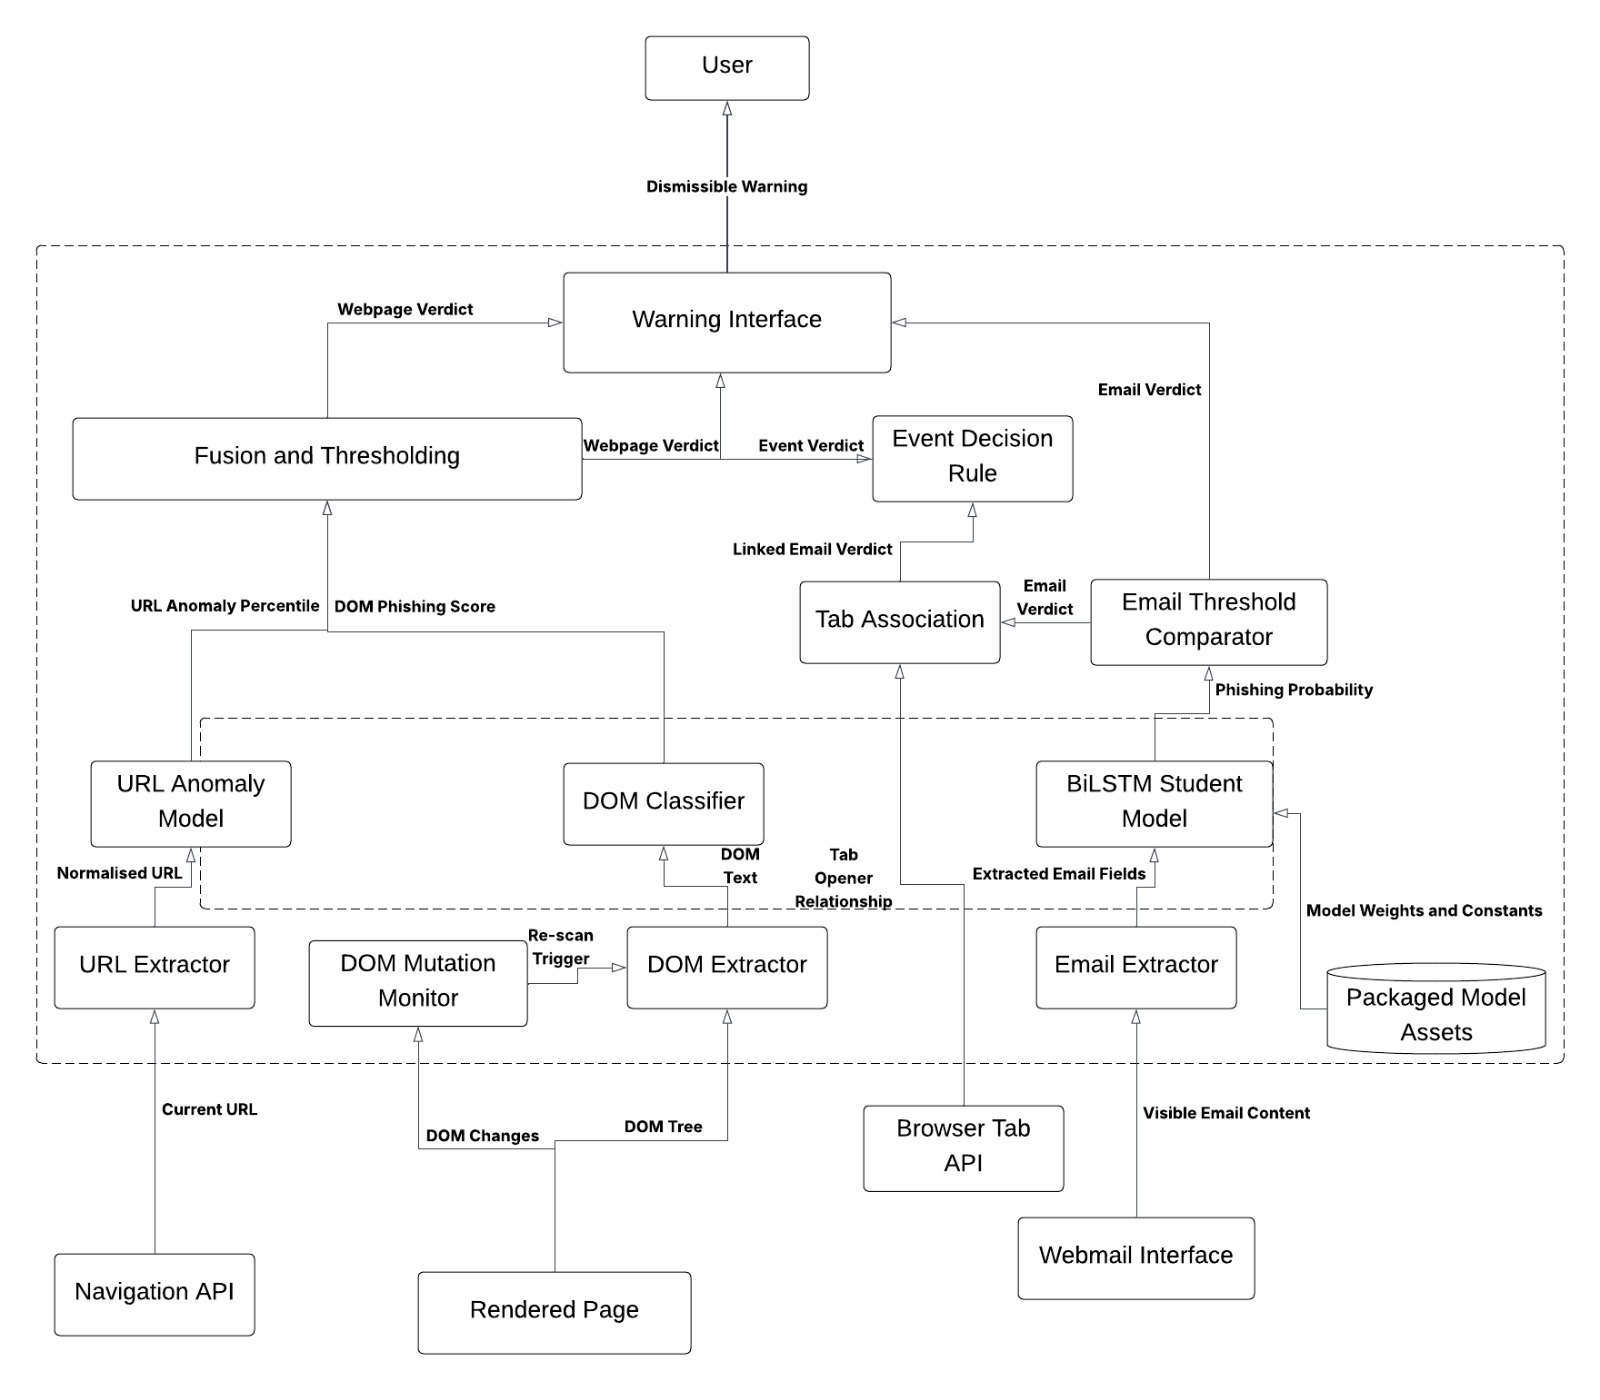
\includegraphics[width=\textwidth]{Figures/fig6.0.png}
    \caption{High-level architecture diagram of PhishHook.}
\end{figure}

The high-level diagram shows the complete system in one view. The URL extractor reads the current URL from the browser navigation API. The DOM extractor reads the rendered DOM. Both feed into the detection pipeline. The URL anomaly model and the DOM classifier produce two scores, which the fusion and thresholding module combines into a verdict.

\section{Subsystem Architecture}
\label{sec:design-subsystems}

This section presents the internal architecture of each subsystem in PhishHook. Each subsystem is shown as a separate diagram with its inputs, internal components, and outputs.

\subsection{URL and DOM Extraction Subsystem}
The URL and DOM extraction subsystem is the first stage of the web pipeline. It reads the current URL from the browser navigation API and reads the rendered page's DOM tree. The URL is passed through a normalisation stage that removes the fragment, lower-cases the scheme and host, and applies the same routine that was used to prepare the training data. The DOM extractor reads the rendered page and extracts the prioritised fields defined in the preprocessing configuration. The extraction controller coordinates both extractors and produces the normalised URL and the DOM-derived text, which are then passed to the URL and DOM models. The same extraction code is used offline to prepare training data, so training and deployment inputs match. Structure of this module is shown in Figure~\ref{fig:extraction}.

\begin{figure}[H]
    \centering
    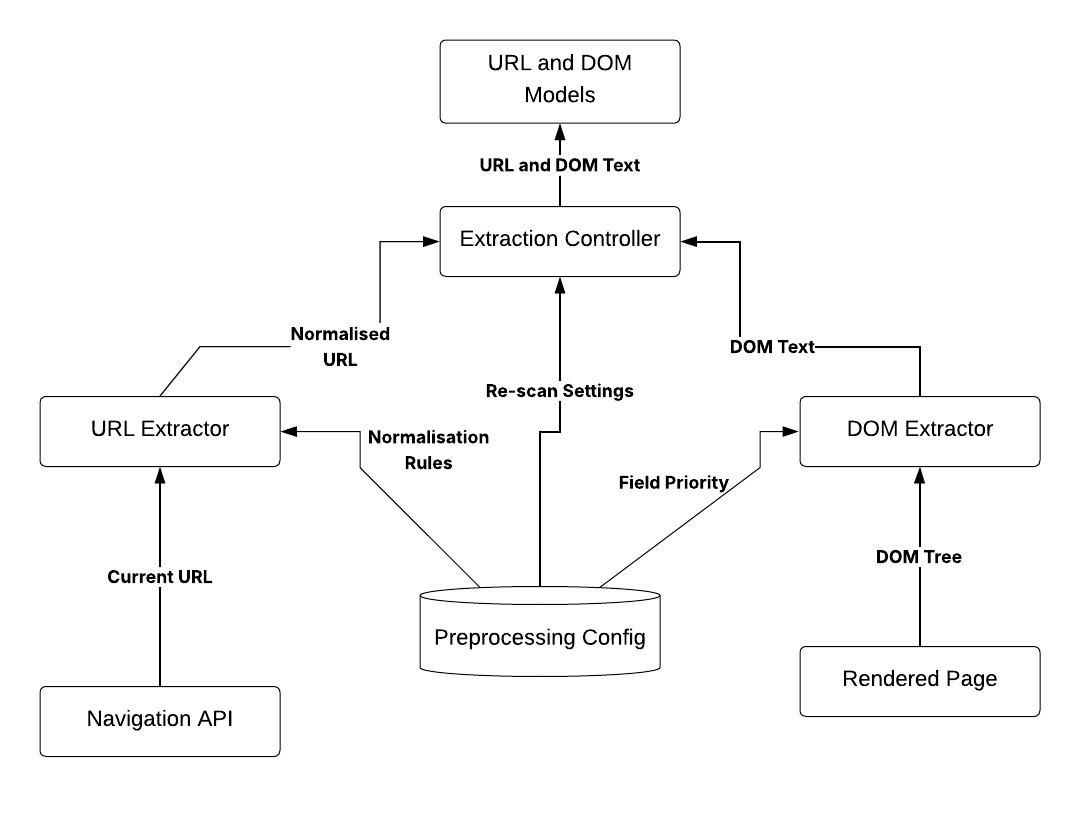
\includegraphics[width=0.85\textwidth]{Figures/fig6.1.png}
    \caption{URL and DOM extraction subsystem.}
    \label{fig:extraction}
\end{figure}

\subsection{Webpage Detection and Score Fusion Subsystem}
The webpage detection and score fusion subsystem combines the outputs of the two web models into a single verdict. The URL anomaly model reads the normalised URL and produces a raw anomaly score, which is converted to a percentile using the frozen benign quantiles shipped with the extension. The DOM classifier reads the DOM-derived text and produces a phishing score. The fusion and thresholding module combines the URL percentile and the DOM phishing score using coefficients and thresholds loaded from the model configuration. The model configuration is stored inside the extension package and is never fetched from a remote server. The result is a webpage verdict that is passed to the warning interface. Structure of this module is shown in Figure~\ref{fig:fusion}.

\begin{figure}[H]
    \centering
    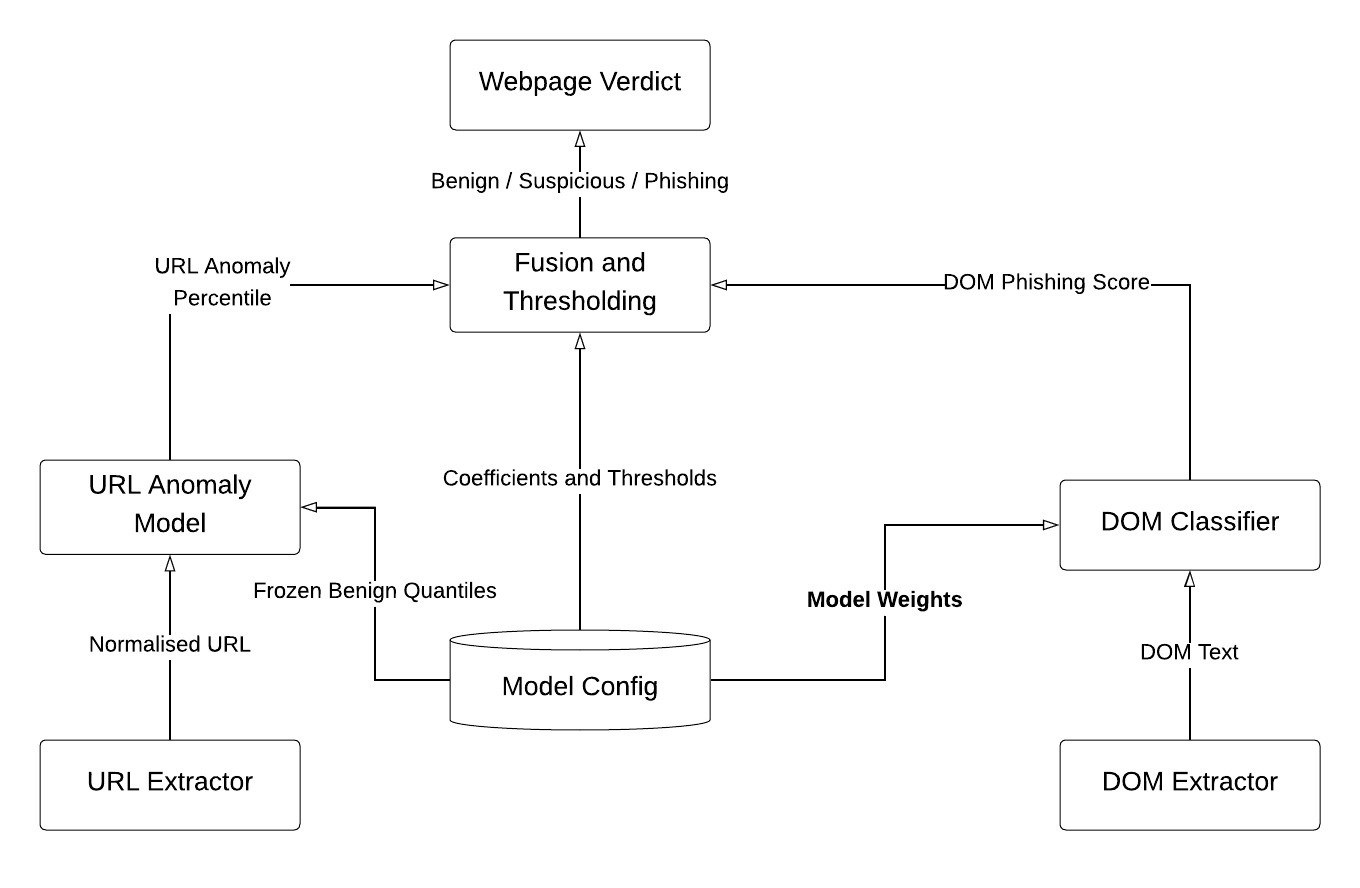
\includegraphics[width=0.85\textwidth]{Figures/fig6.2.png}
    \caption{Webpage detection and score fusion subsystem.}
    \label{fig:fusion}
\end{figure}

\subsection{Email Phishing Detection Subsystem}
The email phishing detection subsystem classifies emails shown in the webmail interface. The email extractor reads visible email content from the webmail interface and produces the extracted email fields, defined in the same way as the training data: subject, visible sender, visible body text, links, and attachment names. The BiLSTM student model reads these fields and produces a phishing probability, which is then thresholded to produce an email verdict. The student model's weights are loaded from the model configuration inside the extension package, so no remote fetch is required. If the webmail DOM cannot be parsed, no verdict is produced rather than a wrong verdict. Structure of this module is shown in Figure~\ref{fig:email}.

\begin{figure}[H]
    \centering
    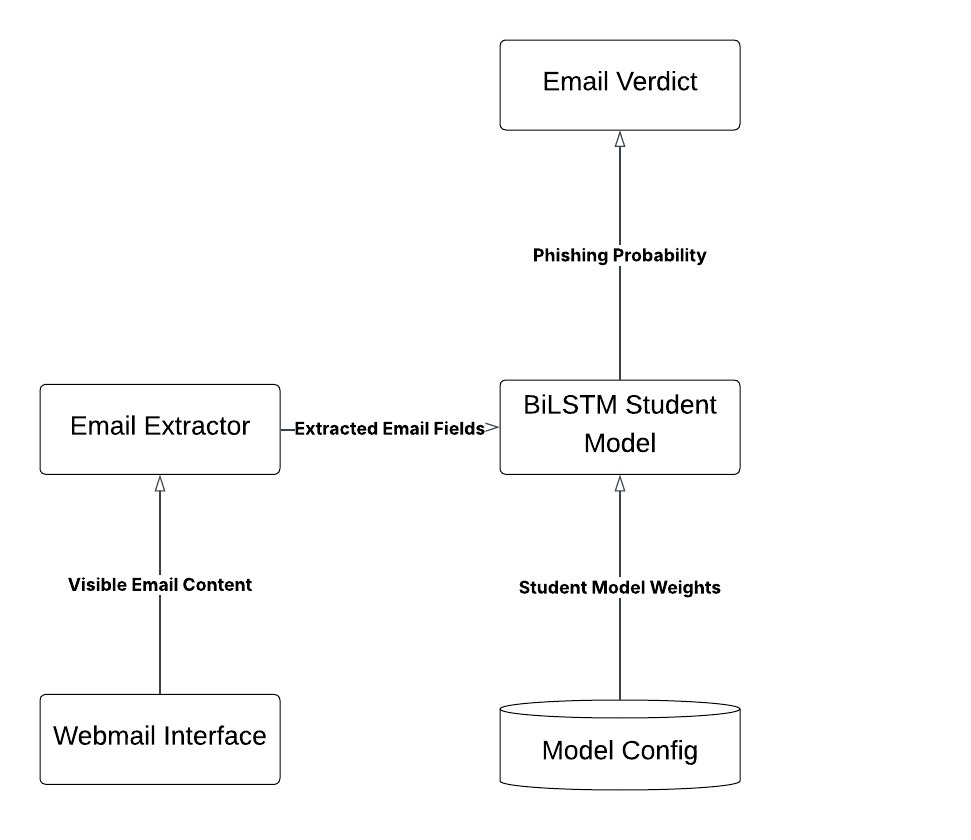
\includegraphics[width=0.85\textwidth]{Figures/fig6.3.png}
    \caption{Email phishing detection subsystem.}
    \label{fig:email}
\end{figure}

\subsection{Dynamic Monitoring and Warning Generation Subsystem}
The dynamic monitoring and warning generation subsystem watches the page for changes after it has loaded and warns the user when a suspicious verdict is produced. The DOM mutation observer watches the rendered page for changes and forwards high-signal changes to the monitoring controller. The monitoring controller uses the window, throttle, and inference cap settings from the monitoring configuration to decide when to trigger a re-scan. When a re-scan is required, the controller sends a re-scan request to the detection pipeline and receives an updated verdict. When the verdict is suspicious or phishing, the controller sends the verdict to the warning interface, which displays a dismissible warning to the user. Structure of this module is shown in Figure~\ref{fig:monitoring}.

\begin{figure}[H]
    \centering
    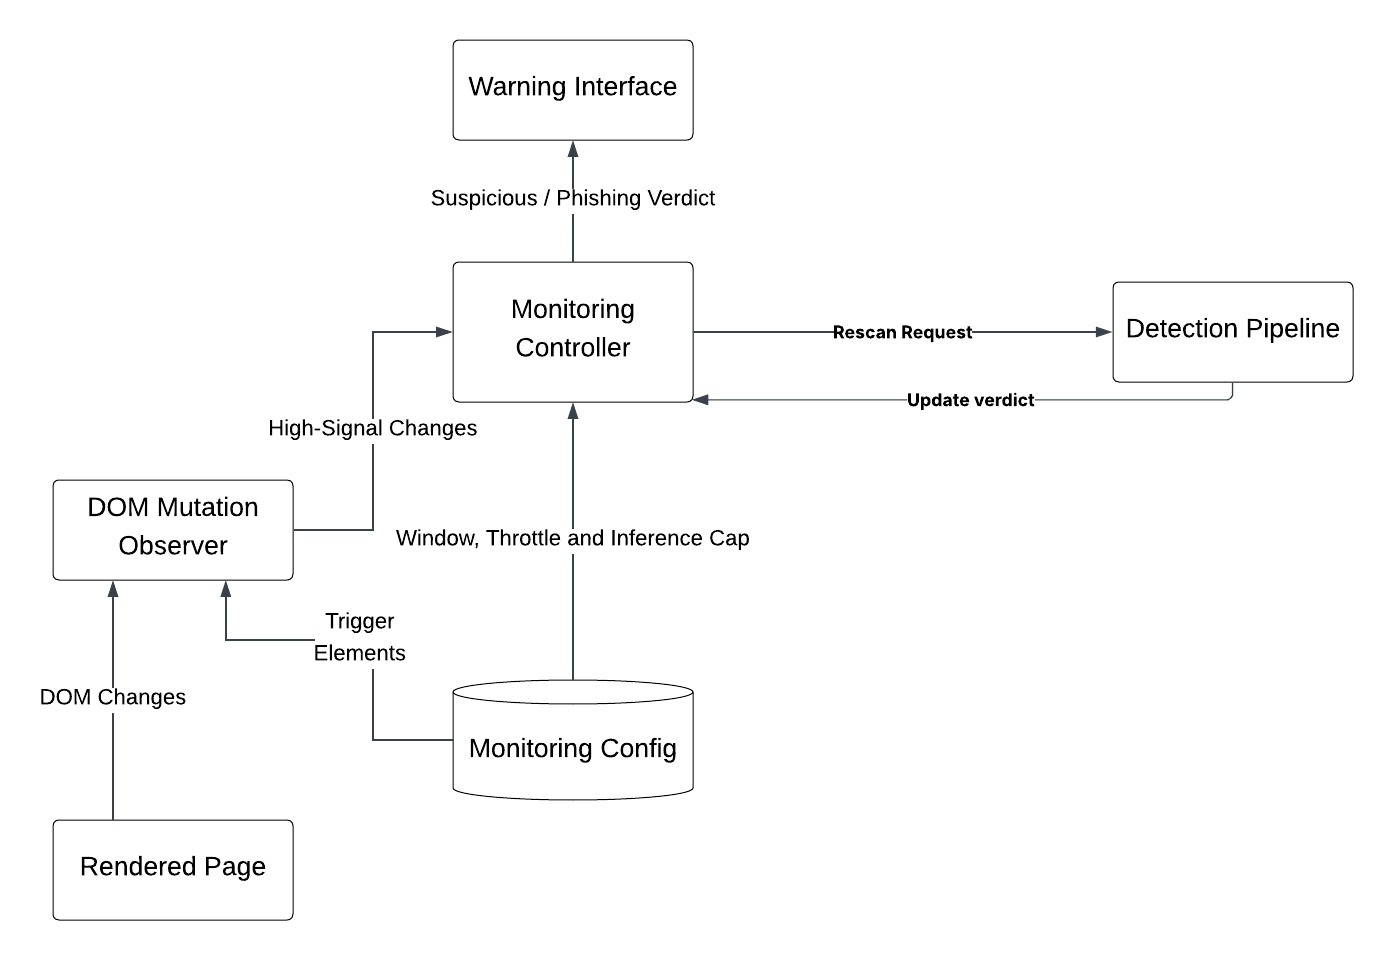
\includegraphics[width=0.85\textwidth]{Figures/fig6.4.png}
    \caption{Dynamic monitoring and warning generation subsystem.}
    \label{fig:monitoring}
\end{figure}

\subsection{Email-to-Web Correlation Subsystem}
The email-to-web correlation subsystem links the verdict on an email to the verdict on the web page it opens. When the user clicks a link inside an open webmail message, the browser tab API provides the tab opener relationship to the tab association module. The tab association module links the email verdict, produced by the email detection module, to the newly opened web page. When both the linked email verdict and the webpage verdict are available within the configured time window, the event decision rule combines them into a single event verdict using the rule and time window from the correlation configuration. If no reliable link exists between the two verdicts, the verdicts remain independent and are not combined. The event verdict is passed to the warning interface and shown to the user. Structure of this module is shown in Figure~\ref{fig:correlation}.

\begin{figure}[H]
    \centering
    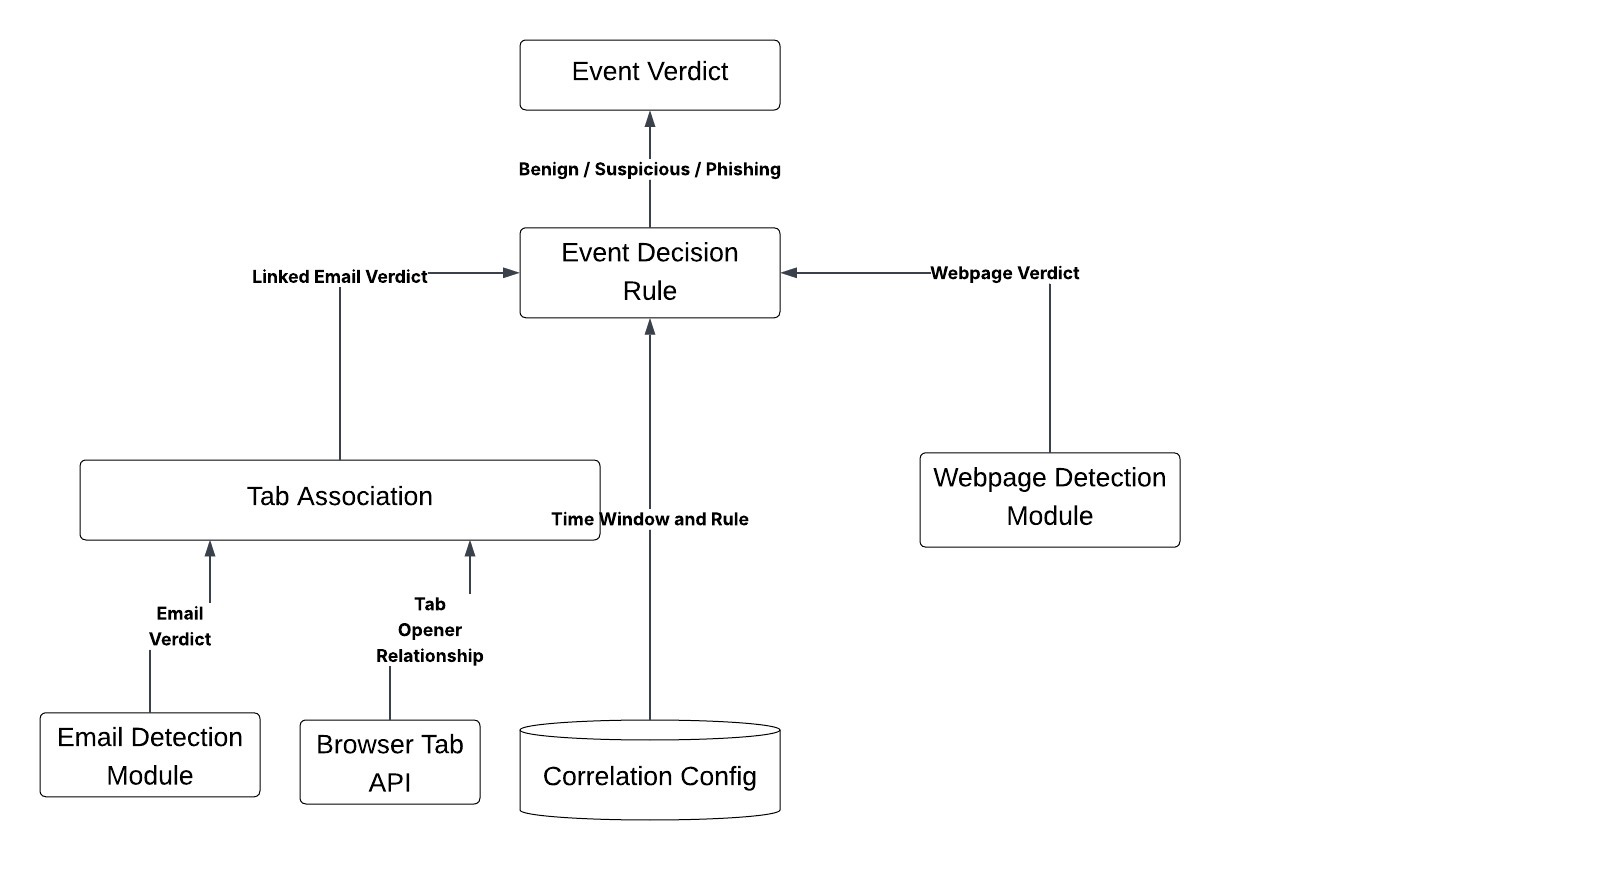
\includegraphics[width=0.85\textwidth]{Figures/fig6.5.png}
    \caption{Email-to-web correlation subsystem.}
    \label{fig:correlation}
\end{figure}

\section{Architectural Strategies}
\label{sec:design-strategies}
The architectural strategies that we will be using for the PhishHook system are given below.

\subsection{Tools and Software}
The extension will be developed using TypeScript and JavaScript, bundled with esbuild. The user interface will use plain HTML and CSS, and the extension will run on Chromium-based browsers using Manifest V3. Model inference inside the browser will use ONNX Runtime Web running through WebAssembly in an offscreen document. Model training and export will be done in Python using PyTorch and ONNX. The URL anomaly module will be implemented with scikit-learn for Isolation Forest and a convolutional autoencoder in PyTorch. The DOM classifier will use MobileBERT. The fusion model will be implemented as a two-input logistic regression. The email student will be a small BiLSTM exported to ONNX. Version control will use GitHub, and system diagrams and GUI mockups will be drawn in Draw.io and Figma. Python's versatility supports training, export, and browser parity tests, ensuring seamless integration across system components.

\subsection{Client-Side Extension Model}
PhishHook adopts a fully client-side model. The browser extension is the only runtime component, and there is no server, no backend, and no cloud inference. The extension consists of four parts: a content script that extracts the URL and the rendered DOM, a service worker that coordinates the analysis, an offscreen document that runs the ONNX models in WebAssembly, and a popup that shows the current verdict. The content script communicates with the service worker using message passing, and the service worker communicates with the offscreen document using the offscreen document API. Communication is asynchronous, so the page is never blocked. This design ensures that all data stays on the user's device.

\subsection{Local Data Handling}
PhishHook does not use a database. There is no persistent storage on the device, and no data is written to disk. Page text, email text, and user identifiers are processed in memory only and discarded once inference is complete. Verdicts and diagnostic counters, when they are needed for event correlation during a session, are held in memory only and are not retained after the browser session ends. This is consistent with the privacy requirement that nothing is stored and nothing is transmitted. If any short-lived state is needed for correlation across tabs, it is kept in the service worker's in-memory store and cleared when the worker is terminated.

\subsection{Interface Paradigms}
The interface employed in this system will prioritise simplicity and non-intrusiveness, ensuring that the extension does not interrupt the user's browsing experience. Each warning will be self-contained, dismissible with one action, and clearly worded. The warning will be rendered in an extension-owned overlay or closed shadow root, so that the page's own scripts cannot read or style it. The extension popup will show the current status and the current page verdict at a glance. Every function will be designed to give the user a clear, meaningful signal without unnecessary detail.

\subsection{Future Plans for Extension}
In the future, several extensions can be explored. The DOM parser can be extended to read content inside cross-origin frames where the browser permits, and to traverse closed shadow roots where a page exposes them. Additional channels such as SMS or QR codes can be added by reusing the same pipeline. Real-time, on-device retraining from user feedback can be considered, subject to privacy constraints. Larger or quantised variants of the DOM classifier can be evaluated for higher accuracy on lower-end devices. The email surface can be extended to more webmail clients. These strategic considerations are poised to enhance problem-solving methodologies and ensure a more comprehensive and reliable solution.

\section{Domain Model / Class Diagram}
\label{sec:domain-model}
Following is the model diagram of the project PhishHook. The diagram shows the two detection surfaces, the web pipeline on top and the email pipeline on the bottom, and how the models and the fusion step are connected.

\begin{figure}[!ht]
    \centering
    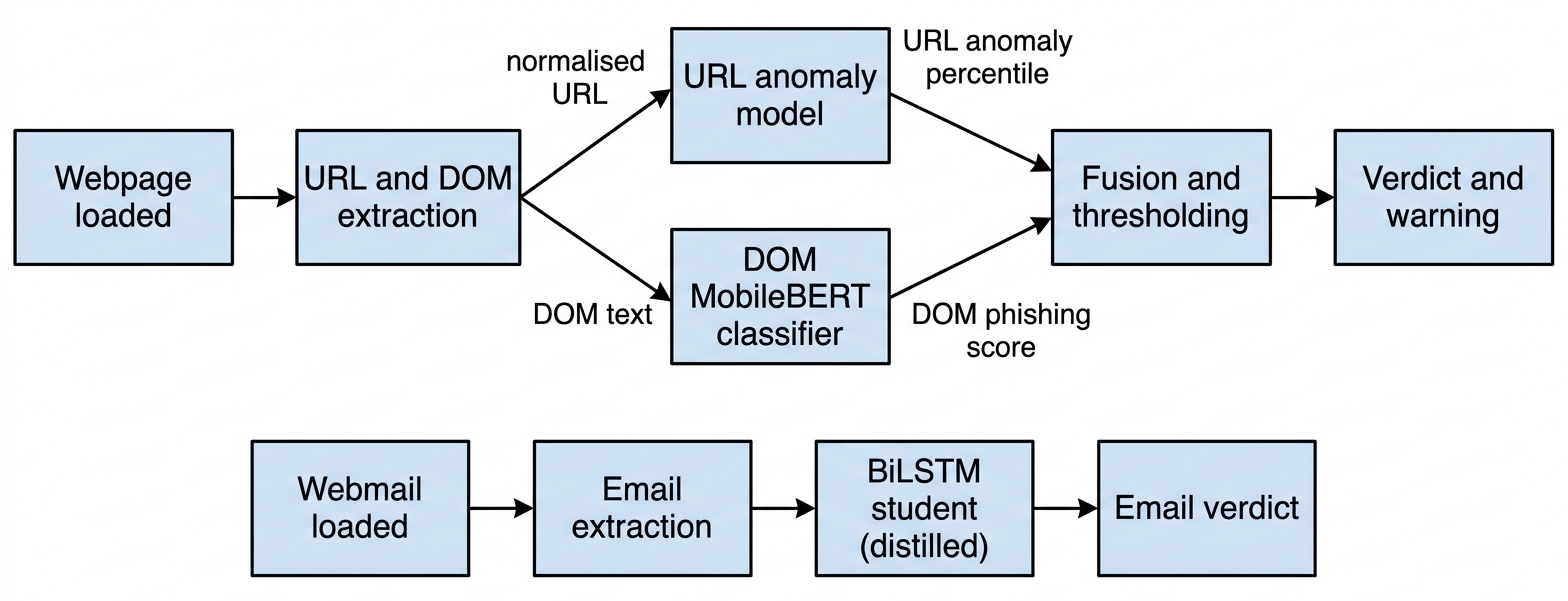
\includegraphics[width=\textwidth]{Figures/model_diagram.png}
    \caption{Model diagram of the PhishHook system.}
    \label{fig:model-diagram}
\end{figure}

The web pipeline begins with the loaded webpage. The URL and DOM extraction step produces a normalised URL and a parsed DOM text. The URL anomaly model and the DOM MobileBERT classifier each produce a score. The fusion and thresholding step combines the two scores and produces the verdict that drives the warning interface. The email pipeline begins with the loaded webmail page. The email extraction step produces the visible email fields, and the distilled BiLSTM student produces the email verdict.


\section{Sequence Diagrams}
\label{sec:sequence-diagrams}
In this section, the sequence diagrams for the main system components are shown along with a description of their working.

\subsection{PhishHook System}
This diagram represents the overall working of the system and shows the sequence of actions triggered when a user loads a web page. The content script extracts the URL and the DOM-derived text, the service worker coordinates the analysis, and the offscreen document runs the URL, DOM, and fusion models.

\begin{figure}[H]
\centering
\begin{tikzpicture}[
    every node/.style={font=\footnotesize, color=black},
    lifeline/.style={draw, dashed, color=black},
    msg/.style={-{Latex}, thick, color=black},
    box/.style={draw, rectangle, minimum width=2.6cm, minimum height=0.8cm, align=center, fill=white, text=black}
]
\node[box] (user) at (0,0) {User};
\node[box] (cs) at (3.2,0) {Content script};
\node[box] (sw) at (6.4,0) {Service worker};
\node[box] (od) at (9.6,0) {Offscreen document};
\draw[lifeline] (user.south) -- ++(0,-8);
\draw[lifeline] (cs.south) -- ++(0,-8);
\draw[lifeline] (sw.south) -- ++(0,-8);
\draw[lifeline] (od.south) -- ++(0,-8);
\draw[msg] (0,-0.9) -- (3.2,-0.9) node[midway,above,font=\scriptsize,color=black]{load page};
\draw[msg] (3.2,-1.8) -- (6.4,-1.8) node[midway,above,font=\scriptsize,color=black]{URL and DOM text};
\draw[msg] (6.4,-2.7) -- (9.6,-2.7) node[midway,above,font=\scriptsize,color=black]{run models};
\draw[msg] (9.6,-3.6) -- (6.4,-3.6) node[midway,above,font=\scriptsize,color=black]{fused score};
\draw[msg] (6.4,-4.5) -- (3.2,-4.5) node[midway,above,font=\scriptsize,color=black]{verdict};
\draw[msg] (3.2,-5.4) -- (0,-5.4) node[midway,above,font=\scriptsize,color=black]{show warning if phishing};
\end{tikzpicture}
\caption{PhishHook system design sequence diagram.}
\label{fig:seq-system}
\end{figure}

\subsection{DOM Parser}
The following diagram represents the working of the DOM parser, initiated once the page has finished loading and its DOM has settled. The parser traverses the rendered DOM, collects the seven element groups, normalises the text, and serialises them in priority order.

\begin{figure}[H]
\centering
\begin{tikzpicture}[
    every node/.style={font=\footnotesize, color=black},
    lifeline/.style={draw, dashed, color=black},
    msg/.style={-{Latex}, thick, color=black},
    box/.style={draw, rectangle, minimum width=2.6cm, minimum height=0.8cm, align=center, fill=white, text=black}
]
\node[box] (page) at (0,0) {Rendered DOM};
\node[box] (parser) at (3.4,0) {DOM parser};
\node[box] (groups) at (6.8,0) {Element groups};
\node[box] (serial) at (10.2,0) {Serialised text};
\draw[lifeline] (page.south) -- ++(0,-6);
\draw[lifeline] (parser.south) -- ++(0,-6);
\draw[lifeline] (groups.south) -- ++(0,-6);
\draw[lifeline] (serial.south) -- ++(0,-6);
\draw[msg] (0,-0.9) -- (3.4,-0.9) node[midway,above,font=\scriptsize,color=black]{traverse};
\draw[msg] (3.4,-3.4) -- (6.8,-3.4) node[midway,above,font=\scriptsize,color=black]{collect seven groups};
\draw[msg] (6.8,-5.8) -- (10.2,-5.8) node[midway,above,font=\scriptsize,color=black]{serialise in priority order};
\end{tikzpicture}
\caption{DOM parser design sequence diagram.}
\label{fig:seq-dom}
\end{figure}

\subsection{URL Anomaly Module}
The diagram illustrates the URL anomaly module's function. When a page loads, the URL is normalised and scored by the deployed model, and its percentile rank is computed from the shipped benign quantiles.

\begin{figure}[H]
\centering
\begin{tikzpicture}[
    every node/.style={font=\footnotesize, color=black},
    lifeline/.style={draw, dashed, color=black},
    msg/.style={-{Latex}, thick, color=black},
    box/.style={draw, rectangle, minimum width=2.6cm, minimum height=0.8cm, align=center, fill=white, text=black}
]
\node[box] (url) at (0,0) {URL string};
\node[box] (norm) at (3.4,0) {URL normaliser};
\node[box] (model) at (6.8,0) {Deployed URL model};
\node[box] (pct) at (10.2,0) {Percentile rank};
\draw[lifeline] (url.south) -- ++(0,-5);
\draw[lifeline] (norm.south) -- ++(0,-5);
\draw[lifeline] (model.south) -- ++(0,-5);
\draw[lifeline] (pct.south) -- ++(0,-5);
\draw[msg] (0,-0.9) -- (3.4,-0.9) node[midway,above,font=\scriptsize,color=black]{normalise};
\draw[msg] (3.4,-1.9) -- (6.8,-1.9) node[midway,above,font=\scriptsize,color=black]{score URL};
\draw[msg] (6.8,-4.3) -- (10.2,-4.3) node[midway,above,font=\scriptsize,color=black]{map against benign quantiles};
\end{tikzpicture}
\caption{URL anomaly module design sequence diagram.}
\label{fig:seq-url}
\end{figure}

\subsection{Email Classification}
The working of the email classification module is represented in the diagram below. When a webmail message is opened, the parser extracts the visible view, and the distilled BiLSTM student classifies it to produce an email verdict.

\begin{figure}[H]
\centering
\begin{tikzpicture}[
    every node/.style={font=\footnotesize, color=black},
    lifeline/.style={draw, dashed, color=black},
    msg/.style={-{Latex}, thick, color=black},
    box/.style={draw, rectangle, minimum width=2.6cm, minimum height=0.8cm, align=center, fill=white, text=black}
]
\node[box] (mail) at (0,0) {Webmail page};
\node[box] (parse) at (3.4,0) {Email parser};
\node[box] (student) at (6.8,0) {BiLSTM student};
\node[box] (verdict) at (10.2,0) {Email verdict};
\draw[lifeline] (mail.south) -- ++(0,-5);
\draw[lifeline] (parse.south) -- ++(0,-5);
\draw[lifeline] (student.south) -- ++(0,-5);
\draw[lifeline] (verdict.south) -- ++(0,-5);
\draw[msg] (0,-0.9) -- (3.4,-0.9) node[midway,above,font=\scriptsize,color=black]{open message};
\draw[msg] (3.4,-1.9) -- (6.8,-1.9) node[midway,above,font=\scriptsize,color=black]{subject, sender, body, links};
\draw[msg] (6.8,-4.3) -- (10.2,-4.3) node[midway,above,font=\scriptsize,color=black]{probability and warning};
\end{tikzpicture}
\caption{Email classification design sequence diagram.}
\label{fig:seq-email}
\end{figure}


\section{Policies and Tactics}
\label{sec:policies}
In the following section, we will delve into specific design policies and tactics employed in the development of the PhishHook system. These decisions are carefully crafted to impact the finer details of the system, focusing on the interface and implementation aspects. Unlike architectural decisions that shape the overall organisation of the system, these policies and tactics influence the intricacies of module implementation. Key considerations discussed here include:

\begin{enumerate}
    \item Algorithm selection for the URL anomaly module.
    \item Algorithm selection for the DOM classifier and the fusion model.
    \item Testing strategy.
    \item Coding guidelines.
    \item Model packaging and update mechanism.
    \item Plans for ensuring requirements traceability.
\end{enumerate}

\subsection{Algorithm Selection for the URL Anomaly Module}
The URL anomaly module is deployed as either a character-level convolutional autoencoder or an Isolation Forest on engineered lexical features. The choice between the two is made by a pre-registered rule on validation data, confirmed on the source-disjoint and temporal test sets. A K-Means distance baseline and a supervised MobileBERT on URL strings are compared offline only, to provide reference points. The unsupervised nature of the deployed model is deliberate: it reflects the observation that labelled phishing URLs are scarce and quickly go stale. The alternative of using only a supervised URL model was considered and rejected because it would duplicate the signals captured by the DOM classifier and would not generalise as well under temporal shift.

\subsection{Algorithm Selection for the DOM Classifier and the Fusion Model}
The DOM classifier uses MobileBERT fine-tuned on the serialised DOM text, exported to int8 ONNX. LightGBM on engineered features are compared offline only. The choice of MobileBERT is driven by its combination of accuracy and small size relative to full BERT models, and by the fact that a quantised version fits within the extension's memory and latency budget. The fusion model uses an L2-regularised logistic regression with two inputs. A tree-based fusion model was considered and rejected because it would overfit the limited calibration and fusion data and would add complexity without a demonstrated benefit.

\subsection{Testing Strategy}
The testing strategy for the system will involve a two-fold approach. A combination of unit testing, integration testing, and real-browser scenario testing will be employed for the extension. Validation and testing of the machine learning modules will be done across the metrics defined in the methodology chapter, including true-positive rate at fixed false-positive rates, precision--recall AUC, calibration error, model size, and latency, with bootstrap confidence intervals and McNemar's test for every comparison. This approach ensures the reliability, credibility, and accuracy of the system as a whole.

\subsection{Coding Guidelines}
Coding guidelines and conventions for TypeScript and Python will be followed for the development of the system. The TypeScript code will follow the official TypeScript style guide, and the Python code will follow PEP~8. Adherence to these guidelines will streamline collaboration among developers and facilitate maintenance of the system in the future.

\subsection{Model Packaging and Update Mechanism}
All models are packaged inside the extension and loaded from local storage through the extension's own resource API. No remote code is fetched at any time. Model updates ship as browser-managed extension updates, in line with the Manifest V3 rule that no remotely hosted code may be executed. Model files and their preprocessing implementations are versioned together, so a new model version always ships with the tokeniser, parser, and fusion constants that were used to train it. This policy ensures that the deployed behaviour matches the trained behaviour.

\subsection{Plans for Ensuring Requirements Traceability}
PhishHook is a research-oriented project, but requirements traceability throughout the project lifecycle will still be ensured. Each system component, feature, and functionality will be linked back to the requirements defined in the Software Requirement Specifications chapter and, where applicable, to the corresponding research question. A traceability matrix will map each functional requirement to the module that implements it, the test case that verifies it, and the chapter section that describes it. This practice keeps the implemented features aligned with the stated requirements and makes the report easier to audit.

\section{Conclusion}
\label{sec:design-conclusion}
In conclusion, this chapter has provided a comprehensive overview of the PhishHook system, covering both its high-level and low-level designs. The architectural strategies, class model, and sequence diagrams together describe how the extension is structured, how data flows between components, and how each detection module interacts with the others. The policies and tactics defined in this chapter fix the algorithm choices, testing strategy, coding standards, packaging rules, and traceability plan that guide the implementation. Collectively, these elements lay the groundwork for the development and implementation of PhishHook.

{
\bibliographystyle{ieeetr}
\bibliography{fypbib}
}


\end{document}